\documentclass[10pt,twocolumn,letterpaper]{article}

\usepackage{cvpr}
\usepackage{times}
\usepackage{epsfig}
\usepackage{graphicx}
\usepackage{amsmath}
\usepackage{amssymb}

% Include other packages here, before hyperref.

% If you comment hyperref and then uncomment it, you should delete
% egpaper.aux before re-running latex.  (Or just hit 'q' on the first latex
% run, let it finish, and you should be clear).
% \usepackage[breaklinks=true,bookmarks=false]{hyperref}
\usepackage{sidecap}
\usepackage{wrapfig}
\usepackage[subrefformat=parens,labelformat=parens]{subcaption} %% provides subfigure
\usepackage{caption}
\usepackage{adjustbox}
\usepackage{float}% If comment this, figure moves
\usepackage{geometry}

% \usepackage{FG2019}
\usepackage{multirow}
\usepackage{graphicx}
\usepackage[acronym]{glossaries}
\usepackage{acronym}

\newcommand{\minitab}[2][c]{\begin{tabular}{#1}#2\end{tabular}}

% symbols for 1/2, etc.
% \usepackage{microtype}      % microtypography
% \usepackage{amsfonts}       % blackboard math symbols
% \usepackage[utf8]{inputenc} % allow utf-8 input
% \usepackage[T1]{fontenc}    % use 8-bit T1 fonts
% % \usepackage{hyperref}       % hyperlinks
% \usepackage[colorlinks = true,
%             linkcolor = blue,
%             urlcolor  = blue,
%             citecolor = blue,
%             anchorcolor = blue]{hyperref}
\usepackage[pagebackref=true,breaklinks=true,letterpaper=true,colorlinks,bookmarks=false]{hyperref}
            
% \usepackage{mathptmx} % assumes new font selection scheme installed
% \usepackage{lipsum}
% \usepackage{slashbox}
\usepackage{booktabs}       % professional-quality tables
%\usepackage{enumitem}
\usepackage [english]{babel}
\usepackage [autostyle, english = american]{csquotes}
\MakeOuterQuote{"}
\usepackage[font=itshape]{quoting}
\usepackage{lipsum}
% \usepackage{subfig}
%% add
\usepackage{graphics}
\usepackage{xcolor}
\usepackage{color, colortbl}
\usepackage{comment}
\usepackage{booktabs, ragged2e}
% \usepackage{arydshln}
% \usepackage{todonotes}
% \usepackage{ctable}
\usepackage{multirow}
\usepackage{makecell}
\usepackage{balance}

\usepackage{pifont}% http://ctan.org/pkg/pifont


\graphicspath{{figures/}} %Setting the graphicspath
\usepackage{bibunits}

\defaultbibliography{bias}
\defaultbibliographystyle{ieee_fullname}

\usepackage[acronym]{glossaries}
\usepackage{acronym}


\usepackage{array}
\newcolumntype{x}[1]{>{\centering\arraybackslash\hspace{0pt}}p{#1}}
\newcommand{\ie}{\textit{i}.\textit{e}., }
\newcommand{\eg}{\textit{e}.\textit{g}., }
\newcommand*{\etc}{etc.\@\xspace}

\newcommand{\xmark}{\ding{56}}%
\newcommand{\checkc}{\ding{51}}%
\newcommand{\NA}{---}

\newacronym{ml}{ML}{machine learning}
\newacronym{fr}{FR}{facial recognition}
\newacronym{fv}{FV}{facial verification}

\newacronym{cnn}{CNN}{convolutional neural network}
\newacronym{nn}{NN}{neural network}
\newacronym{mtcnn}{MTCNN}{\emph{multi-task \gls{cnn}}}

\newacronym{gan}{GAN}{generative adversarial network}
\newacronym{se}{SE}{\emph{Squeeze-and-Excitation}}
\newacronym{d}{$D$}{discriminator}
\newacronym{g}{$G$}{generator}
\newacronym{dbvae}{DB-VAE}{Debiasing Variational Autoencoder}


\newacronym{lut}{LUT}{Look-Up-Table}
\newacronym{soa}{SOTA}{state-of-the-art}

\newacronym{fiw}{FIW}{Families In the Wild}
\newacronym{lfw}{LFW}{Labeled Faces in the Wild}
\newacronym{bfw}{BFW}{Balanced Faces In the Wild}
\newacronym{rfw}{RFW}{Racial Faces in-the-Wild:}
\newacronym{dp}{DemogPairs}{Demographic Pairs}
\newacronym{itwcc}{ITWCC}{Wild Child Celebrity}

\newacronym{m}{M}{\textit{Male}}
\newacronym{f}{F}{\textit{Female}}
\newacronym{a}{A}{\textit{Asian}}
\newacronym{b}{B}{\textit{Black}}
\newacronym{i}{I}{\textit{Indian}}
\newacronym{w}{W}{\textit{White}}
\newacronym{af}{AF}{\textit{Asian}-\textit{Female}}
\newacronym{am}{AM}{\textit{Asian}-\textit{Male}}
\newacronym{bf}{BF}{\textit{Black}-\textit{Female}}
\newacronym{bm}{BM}{\textit{Black}-\textit{Male}}
\newacronym{if}{IF}{\textit{Indian}-\textit{Female}}
\newacronym{im}{IM}{\textit{Indian}-\textit{Male}}
\newacronym{wf}{WF}{\textit{White}-\textit{Female}}
\newacronym{wm}{WM}{\textit{White}-\textit{Male}}


\newacronym{fd}{FD}{Face Discrimination}
\newacronym{bb}{BB}{bounding box}

\newacronym{sdm}{SDM}{signal detection model}
\newacronym{roc}{ROC}{receiver operating characteristic}
\newacronym{nmse}{NMSE}{Normalized Mean Square Error}
\newacronym{det}{DET}{Detection error trade-off}
\newacronym{tp}{TP}{true-positive}
\newacronym{fp}{FP}{false-positive}

\newacronym{tpir}{TPIR}{true-positive identification rate}
\newacronym{frir}{FRIR}{false-reject identification rate}
\newacronym{fpir}{FRIR}{false-positive identification rate}

\newacronym{fn}{FN}{false-negative}
\newacronym{frr}{FRR}{false-reject rate}
\newacronym{fnr}{FNR}{false-negative rate}

\newacronym{fpr}{FPR}{false-positive rate}

\newacronym{tpr}{TPR}{true-positive rate}


\newacronym{tar}{TAR}{True Acceptance Rate}
\newacronym{far}{FAR}{False Acceptance Rate}
\newacronym{eer}{EER}{Equal Error Rate}

\newacronym{cs}{CS}{Cosine Similarity}


\newacronym{lime}{LIME}{Local Interpretable Model-Agnostic Explanations}
\newacronym{nas}{NAS}{Neural Architecture Search}
\newacronym{gapf}{GAPF}{Generative Adversarial Privacy and Fairness}

                                                         % paper
%\setlist[itemize]{leftmargin=*}
\newcommand{\ra}[1]{\renewcommand{\arraystretch}{#1}}
\newcommand{\mc}[2]{\multicolumn{#1}{c}{#2}}
\definecolor{Gray}{gray}{0.85}
\definecolor{LightCyan}{rgb}{0.88,1,1}

\newcolumntype{a}{>{\columncolor{Gray}}c}
\newcolumntype{b}{>{\columncolor{white}}c}
\renewcommand{\arraystretch}{1.4}
%\newcommand{\xmark}{\ding{53}}%

\newcommand{\highlightb}[1]{%
\colorbox{blue!30}{$\displaystyle#1$}}
\newcommand{\vo}{\vec{o}\@ifnextchar{^}{\,}{}}

\newcommand{\vx}{\vec{x}\@ifnextchar{^}{\,}{}}

% \let\vec\mathbf
% \usepackage[T1]{fontenc}
% \usepackage[latin9]{inputenc}

\def\colorModel{hsb} %You can use rgb or hsb
\usepackage{babel}
\usepackage[table]{xcolor}
\usepackage{collcell}
\def\colorModel{hsb} %You can use rgb or hsb

\usepackage{hhline}
\newcommand\ColCell[1]{
  \pgfmathparse{#1<50?1:0}  %Threshold for changing the font color into the cells
    \ifnum\pgfmathresult=0\relax\color{white}\fi
  \pgfmathsetmacro\compA{0}      %Component R or H
  \pgfmathsetmacro\compB{#1/100} %Component G or S
  \pgfmathsetmacro\compC{1}      %Component B or B
  \edef\x{\noexpand\centering\noexpand\cellcolor[\colorModel]{\compA,\compB,\compC}}\x #1
  } 
\newcolumntype{E}{>{\collectcell\ColCell}m{0.4cm}<{\endcollectcell}}  %Cell width
\newcommand*\rot{\rotatebox{90}}

% \cvprfinalcopy % *** Uncomment this line for the final submission

\def\cvprPaperID{0001} % *** Enter the CVPR Paper ID here
\def\httilde{\mbox{\tt\raisebox{-.5ex}{\symbol{126}}}}

% Pages are numbered in submission mode, and unnumbered in camera-ready
\ifcvprfinal\pagestyle{empty}\fi
%\setcounter{page}{4321}
\begin{document}

%%%%%%%%% TITLE
\title{Face Recognition: Too Bias, or Not Too Bias?}

% \author{First Author\\
% Institution1\\
% Institution1 address\\
% {\tt\small firstauthor@i1.org}
% % For a paper whose authors are all at the same institution,
% % omit the following lines up until the closing ``}''.
% % Additional authors and addresses can be added with ``\and'',
% % just like the second author.
% % To save space, use either the email address or home page, not both
% \and
% Second Author\\
% Institution2\\
% First line of institution2 address\\
% {\tt\small secondauthor@i2.org}
% }

\maketitle
%\thispagestyle{empty}

%%%%%%%%% ABSTRACT
\begin{abstract}
We reveal critical insights into problems of bias in state-of-the-art \gls{fr} systems using a novel \gls{bfw} dataset: data balanced for gender and ethnic groups. We show variations in the optimal scoring threshold for face-pairs across different subgroups. Thus, the conventional approach of learning a  global threshold for all pairs resulting in performance gaps among subgroups. By learning subgroup-specific thresholds, we not only mitigate problems in performance gaps but also show a notable boost in the overall performance. Furthermore, we do a human evaluation to measure the bias in humans, which supports the hypothesis that such a bias exists in human perception. For the \gls{bfw} database, source code, and more, visit \href{http://cvpr2020.thecvf.com/submission/main-conference/author-guidelines#policies}{github}.
% \href{https://github.com/visionjo/facerec-bias-bfw}{github.com/visionjo/facerec-bias-bfw}
\end{abstract}


%%%%%%%%%%%%%%%%%%%%%%%%%%%%%%%%%%%%%%%%%%%%%%%%%%%%%%%%%%%%%%%%%%%%%%%%%%%%%%%%
% \begin{bibunit}

\glsresetall
\section{Introduction}
    As more of society becomes integrated with \gls{ml}, bias, fairness, and the formalization of \gls{ml} standards attract more attention~\cite{10.1007/978-3-030-13469-3_68, anne2018women, wang2018racial}. Thus, an effect of the growing dependency on \gls{ml} are growing concerns for biased and unfair algorithms, \eg untrustworthy and racist \gls{fr} systems~\cite{england2019,snow2018}.
    


    Typically, \glspl{cnn} are trained on faces identified by a detection system. Specifically, for \gls{fr}, the goal is to encode faces in an N-dimensional space such that samples of the same identity are neighbors and those of different identity of further apart. Thus, the goal is to identify subjects with face encodings. We can deploy a \gls{cnn} to encode faces, and then compare via a similarity score: assume pairs with a high enough score are \emph{genuine}; else, an \emph{imposter}. 

% \begin{figure}
%     \centering
%     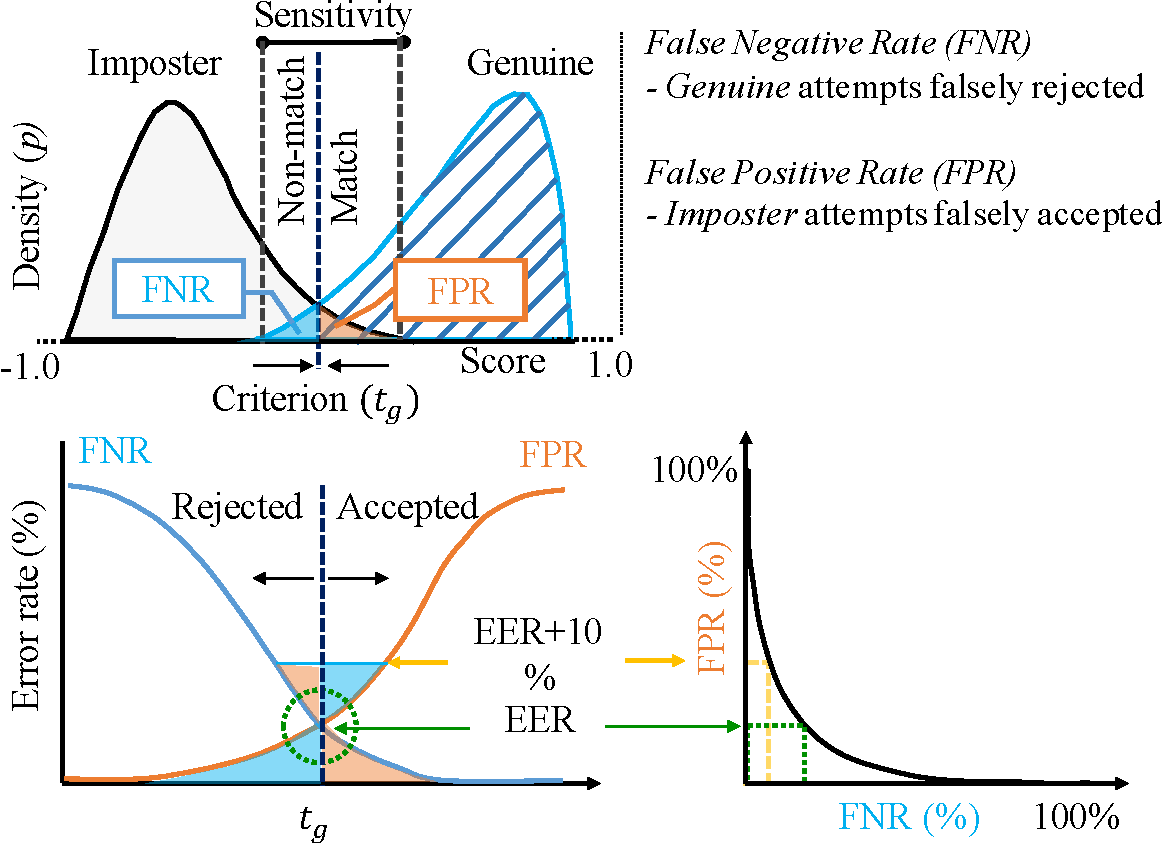
\includegraphics[width=\linewidth]{figures/fig1-crop.pdf}
%     \caption{Caption}
%     \label{fig:my_label}
% \end{figure}
    \begin{figure}[t!]
        \centering
        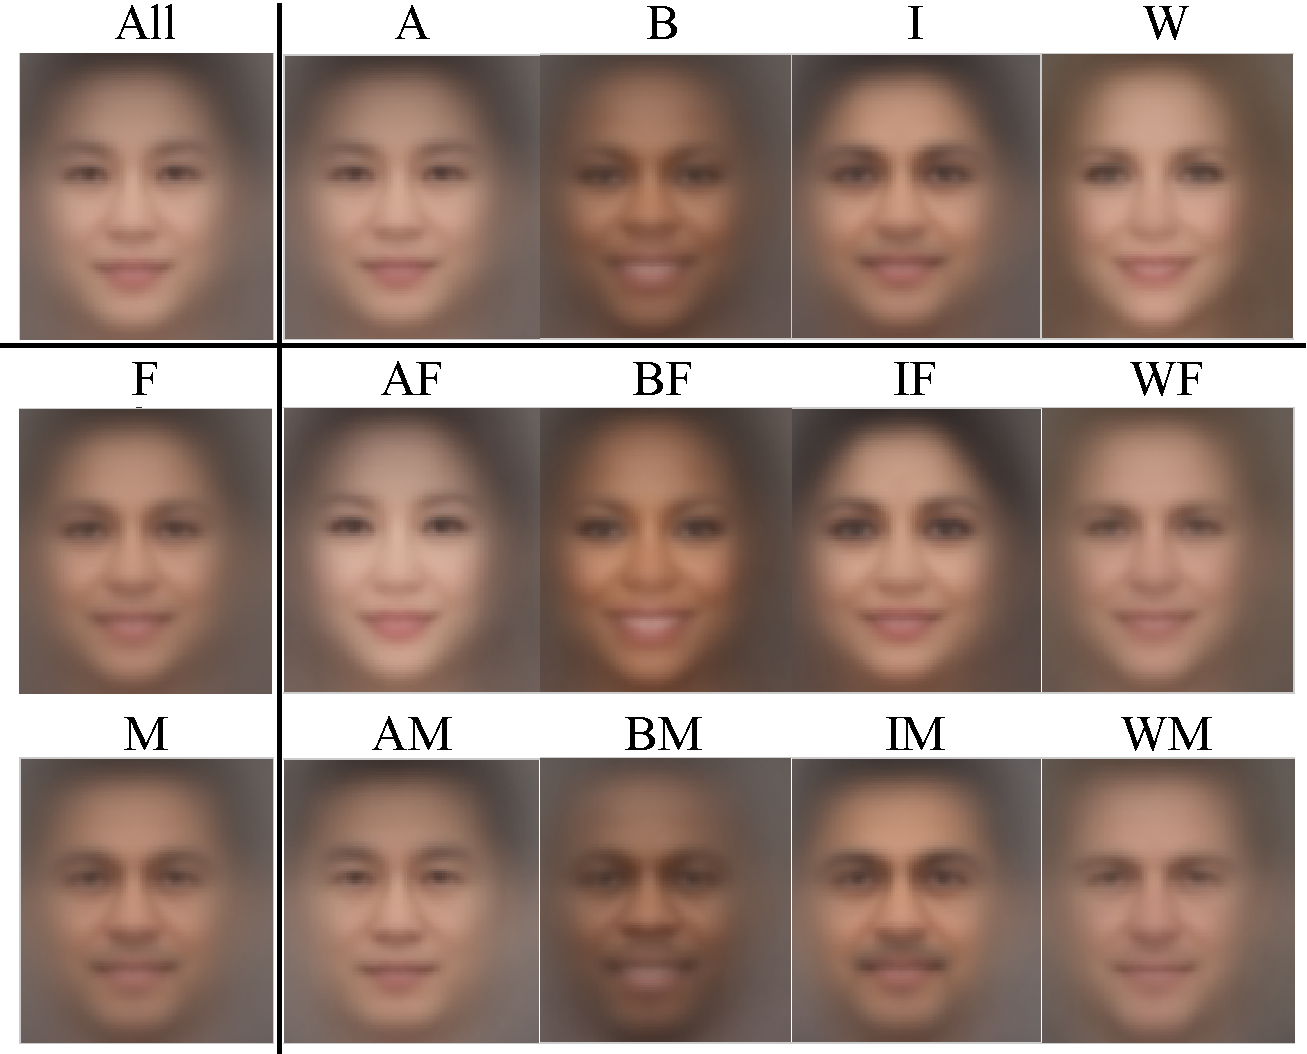
\includegraphics[width=.8\linewidth]{figures/montage.pdf}
        \caption{\small{\textbf{\gls{bfw}.} Average face of the different subsets: \emph{top-left}: the entire \gls{bfw}; \emph{top-row} per race;  \emph{left-column}: per gender. The others represent the ethnicity and gender of the race and gender, respectively. Table~\ref{tab:ethnic-splits} defines the acronyms of subgroups.}}
        \label{fig:avg-faces}
    \end{figure}
    
    When comparing scores, typically, a fixed threshold sets the decision boundary. Thus, features of the same identity must satisfy a criterion via a single value~\cite{deng2019arcface, liu2017sphereface, wang2018additive, wang2018cosface}. However, we found that a single (\ie global) threshold is a crude measure that leads to skewed errors - the held-out set used to determine the threshold tends to share the same distribution with the test data, which favors specific demographics that are a majority. That skew, the difference in the performance of an algorithm of certain demographics, is our definition of bias. A key question is: \emph{is \gls{fr} too biased, or not?} 
    

\begin{table*}[!t]
    \centering
    \caption{\small{\textbf{Database stats and nomenclature, optimal thresholds ($t_o$), and accuracy scores.} \textit{Header:} Subgroup definitions. \textit{Top-row:} Statistics of \gls{bfw}. \textit{Middle:} Number of pairs for each partition. \textit{Bottom:} Accuracy with a global threshold $t_g$, the optimal threshold $t_o$, and accuracy with $t_o$ per subgroup. Specifically, $t_g$=0.259$\pm$0.002 when averaged across the five folds. Columns grouped by race and then further split by gender. Out of millions of pairs, accuracy is inconsistent across subgroups. Furthermore, $F$ tends to perform inferior to that of $M$ for all but B.}}\label{tab:ethnic-splits}
    \scalebox{.75}{
     \resizebox{\textwidth}{!}{%
    \begin{tabular}{r c c c c c c c c l}
        \toprule
        & \multicolumn{2}{c}{Asian (A)} & \multicolumn{2}{c}{Black (B)}  & \multicolumn{2}{c}{Indian (I)}& \multicolumn{2}{c}{White (W)}\\
        \cmidrule(l){2-3} \cmidrule(l){4-5} \cmidrule(l){6-7}\cmidrule(l){8-9} % spanning less than the full width of the table - you can add (r) or (l) just before the opening curly bracket to shorten the rule on the left or right side
         & Female (AF) & Male (AM) & BF & BM& IF & IM & WF & WM&Aggregated\\ % Column names row
        \midrule

       \# Faces  &  2,500&  2,500& 2,500 & 2,500& 2,500 & 2,500 & 2,500 & 2,500 &20,000 \\ % row 1
        \# Subjects & 100& 100& 100  & 100  & 100  & 100& 100 &100&800  \\ % row 2
        \# Faces / Subject  & 25 & 25    & 25 & 25 & 25  & 25  &  25 & 25 & 25\\ % row 3
        % \midrule
\specialrule{.01em}{.05em}{.05em}
            \# Positive Pairs &  30,000&  30,000& 30,000 &30,000 & 30,000 &30,000&30,000 & 30,000 &240,000 \\ % row 1
        \# Negative Pairs & 85,135&  85,232& 85,016  & 85,141  & 85,287  & 85,152& 85,223 &85,193&681,379  \\ % row 2

        \# Pairs (Total) & 115,135 & 115,232    &115016 &115,141 & 115287  & 115,152  &  115,223& 115193 & 921,379\\ % row 3
        % \midrule
        % \specialrule{.01em}{.05em}{.05em}
        % Acc$@t_g$ & 0.941 & 0.952  & 0.967 & 0.960 & 0.958 &0.962  & 0.973 & 0.981 &0.962 $\pm$0.012 \\
        % $t_o$ & 0.255 &  0.246 & 0.277 &0.242  &0.297 & 0.264& 0.233 &0.239 &0.257$\pm$0.006\\ % row 4
        
        % Acc$@t_o$ & 0.942 &0.952 &0.968 &0.961 &0.960 &0.962 & 0.974 &0.982 & 0.963 $\pm$ 0.012\\
        \bottomrule
    \end{tabular}}
    % \glsunset{af}
    }
    % % \glsunset{af}
    % \glsunset{am}
    % \glsunset{bf}
    % \glsunset{bm}
    % \glsunset{if}
    % \glsunset{im}
    % \glsunset{wf}
    % \glsunset{wm}
    % \vspace{-12pt}
\end{table*}

    
    Making matters more challenging is that race and ethnicity are loosely defined. For example, the US Census Bureau allows an individual to self-identify race.\footnote{\scriptsize\href{https://www.census.gov/mso/www/training/pdf/race-ethnicity-onepager.pdf}{www.census.gov/mso/www/training/pdf/race-ethnicity-onepager}} For this work, we define subgroups as specific sub-populations with face characteristics similar to those found in a region. 
    
    
    The adverse effects of a global threshold are two-fold: \textbf{(1)} the mapping produced by a \gls{cnn} is nonuniform. Therefore, distances between pairs of faces in different demographics vary in distribution of similarity scores (Fig~\ref{fig:detection-model}); \textbf{(2)} the evaluation set is imbalanced as well. Particular demographics making up a majority of the population will carry most weight on the reported performance ratings. Reported results favor the common traits over the underrepresented. Alas, demographics like gender, ethnicity, race, and age are underrepresented in most public datasets~\cite{merler2019diversity, wang2018racial}. 
    
    % The result is various types of biases in FR systems in favor of or against particular demographics remain a question.
    
    For \textbf{(1)} we propose subgroup-specific (\ie optimal) thresholds; to address \textbf{(2)}, we introduce a new benchmark for measuring bias in \gls{fr}, \gls{bfw} (Table~\ref{tab:compared} \&~\ref{tab:ethnic-splits}). \gls{bfw} allows for a fair evaluation of \gls{fr} systems, while enabling demographic-specific ratings to be reported. We use \gls{bfw} to gain a deeper understanding of the extent of bias present in \gls{soa} \gls{cnn} used to encode faces. Then, we suggest a mechanism to mitigate problems of bias with more balanced performance ratings for different demographics. Specifically, we propose using an adaptive threshold that varies depending on the characteristics of detected facial attributes (\ie gender and ethnicity, Fig~\ref{fig:avg-faces}). We show an increase in accuracy with a balanced performance for different subgroups. Similarly, we show a positive effect of adjusting the similarity threshold based on the facial features of matched faces. Thus, selective use of similarity thresholds in current \gls{soa} \gls{fr} systems provides more intuition in \gls{fr} research with a method easy to adopt in practice. 
    
    
    The contributions of this work are 3-fold. (1) We built a balanced dataset as a proxy to measure verification performance per subgroup for studies of bias in \gls{fr}. (2) We revealed an unwanted bias in scores of face pairs - a bias that causes ratings to skew across demographics. For this, we showed that an adaptive threshold per subgroup balances performance (\ie the typical use of a global threshold unfavorable, which we address via optimal thresholds). (3) We surveyed humans to demonstrate bias in human perception.\footnote{NIH-certified, \textit{Protect Humans in Research}.}%19-09-08}.}
    % \begin{enumerate}
    %     \item Built a balanced dataset as a proxy to measure verification performance per subgroup.
    %     \item Analyzed an unwanted bias in scores of face pairs while showing that optimal thresholds determined per subgroup significantly boost and balance performances.
    %     \item Showed bias causes inconsistencies in ratings across demographics-- the typical use of a global threshold unfavorable. We mitigate the problem via adaptive thresholds.
    %     \item Conducted human-evaluations to demonstrate bias in human perception.\footnote{NIH-certified, \textit{Protect Humans in Research}, \textcolor{red}{IRB 19-09-08}.}
    % \end{enumerate}


\section{Background Information}
    \subsection{Bias in \gls{ml}}
        The progress and the commercial value of \gls{ml} is exciting; however, the trust of society in \gls{ml} will take time to build due to inherent biases. The exact definitions and implications of bias vary between sources, as do its sources and types. A common theme is that bias hinders performance ratings in ways that skew to a particular sub-population-- the source varies, whether from humans~\cite{windmann1998subconscious}, data and label types~\cite{tommasi2017deeper}, \gls{ml} models~\cite{amini2019uncovering, kim2019learning}, or evaluation protocols~\cite{stock2018convnets}. For instance, a vehicle-detection model might miss cars if training data was mostly trucks. In practice, many \gls{ml} systems learn on biased data, which could be detrimental for society. 


    \subsection{Bias in \gls{fr}}
        Problems of bias in \gls{fr} have been driven by different motivations; therefore, solutions have been posed for different matters. To name a few: data augmentation~\cite{yin2019feature}, one-shot learning~\cite{ding2018one}, demographic parity and fairness with priority on privacy~\cite{huang2018generative}, domain adaptation~\cite{wang2018racial}, differences in face-based attributes across demographics~\cite{wang2018they}, and even data exploration~\cite{muthukumar2019}. Yin~\etal proposed to augment the feature space of underrepresented classes using other classes with a diverse collection of samples to encourage distributions of underrepresented classes to more closely resemble that of the others~\cite{yin2019feature}. Similarly, others formulated the imbalanced class problem as one-shot learning, where a \gls{gan} was trained to generate face features to augment classes with fewer samples~\cite{ding2018one}. \gls{gapf} was proposed to create fair representations of the data in a quantifiable way, allowing for the finding of a de-correlation scheme from the data without access to its statistics~\cite{huang2018generative}. Wang~\etal defined subgroups at a finer-level (\ie Chinese, Japanese, Korean), and determined the familiarity of faces inter-subgroup~\cite{wang2018they}. Genders have also been used to make subgroups (\eg for analysis of gender-based face encodings~\cite{muthukumar2019}). Most recently,~\cite{wang2018racial} proposed adapting domains to bridge the bias gap by knowledge transfer, which was supported by a novel data collection, \gls{rfw}. The release of \gls{rfw} occurred after \gls{bfw} was built - although similar in terms of demographics, \gls{rfw} uses faces from MSCeleb~\cite{guo2016ms} for testing, and assumes CASIA-Face~\cite{yi2014learning} and VGG2~\cite{Cao18} were used to train. In contrast, our \gls{bfw} assumes VGG2 as the test set. 
        % As shown in \cite{wang2018racial}, MSCeleb is highly imbalanced, primarily consisting of images of white individuals. 
        % For this, we expect bias from data, for this is the training set. 
        Furthermore, \gls{bfw} balances gender and race: \gls{rfw} splits subgroups by gender and race, while \gls{bfw} has gender, race, or both). 
        % Thus, \gls{rfw} and \gls{bfw} complement one another. % - both add demographic for subjects with faces in renowned, large-scale \gls{fr} datasets.

    
Most similar to us is~\cite{das2018, demogPairs, lopez2019dataset, srinivas2019face} - each were motivated by insufficient paired data for studying bias in \gls{fr}; then, problems were addressed using labeled data from existing image collections. Specifically, Hupont~\etal curated a set of faces based on racial demographics (\ie \gls{a}, \gls{b}, and \gls{w}) called \gls{dp}~\cite{demogPairs}, while~\cite{srinivas2019face} honed in on adults versus children called \gls{itwcc}. Like the proposed \gls{bfw}, both were built by sampling existing databases, but with the addition of tags for the respective subgroups of interest. Besides, the additional data of \gls{bfw} (\ie added an additional subgroup \gls{i}, along with additional subjects with more faces for all subgroups), we also further split subgroups by gender. Furthermore, we focus on the problem of facial verification and the different levels of sensitivity in cosine similarity scores per subgroup.

    \begin{table*}[t!]
        
        \centering
        \caption{\small{\textbf{\gls{bfw} compared to related datasets.} Our \gls{bfw} is balanced across ID, gender, and ethnicity (Table~\ref{tab:ethnic-splits}). Compared with \gls{dp}, \gls{bfw} provides more samples per subject and subgroups per set, while only using a single resource, VGG2. \gls{rfw}, on the other hand, supports a different task (\ie domain adaptation), and focuses on race-distribution, but not the distribution of identities.}}
        \scriptsize
        \begin{tabular}{rccccccc}%x{10mm}x{3mm}x{10mm}x{8mm}}%\toprule
        
            \multicolumn{2}{c}{Database} & \multicolumn{3}{c}{Number of}& \multicolumn{3}{c}{Balanced Labels}\\
            \cmidrule(lr){1-2}	\cmidrule(lr){3-5} \cmidrule(lr){6-8}
            Name & Source Data & Faces &  IDs & Subgroups & ID & Ethnicity & Gender\\\midrule
            \gls{dp}~\cite{demogPairs}     & CASIA-W~\cite{yi2014learning}, VGG~\cite{schroff2015facenet} \&VGG2~\cite{Cao18} & 10,800& 600 & 6 &\checkc& \checkc &\checkc \\
            \gls{rfw}~\cite{wang2018racial}     &  MS-Celeb-1M &$\approx$80,000&$\approx$12,000& 4 & \xmark & \checkc &\xmark \\
            \gls{bfw} (ours) & VGG2 & 20,000 & 800 &8 & \checkc & \checkc &\checkc \\\bottomrule
        \end{tabular}
        \label{tab:compared}
    \end{table*}
    
\subsection{Human bias in \gls{ml}}
Bias is not unique to \gls{ml} - humans are also susceptible to a perceived bias. In fact, biases exist across race, gender, and even age~\cite{10.1007/978-3-030-13469-3_68, bar2006, meissner2001, nicholls2018}. Wang~\etal showed machines surpass human performance in discriminating between Japanese, Chinese, or Korean faces by nearly 150\%~\cite{wang2018they}, as humans just pass random (\ie 38.89\% accuracy).

We expect human bias to skew to their own genders and races. For this, we measure the human perception with face pairs of different subgroups (Section~\ref{subsec:human-assessment}). The results concur with~\cite{wang2018they}, as we also recorded overall averages below random ($<$50\%). %The details on settings and number of submissions per demographics are discussed in Section~\ref{}.



\glsunset{if}\glsunset{im}\glsunset{af}\glsunset{am}\glsunset{bf}\glsunset{bm}\glsunset{wf}\glsunset{wm}
\section{The BFW Benchmark and Dataset}


We now discuss the \gls{bfw} dataset (\ie collection and preparation), along with the evaluation protocols. We conclude this section by reviewing the settings followed to survey bias in humans.

\subsection{The data}
Problems of bias in \gls{fr} motivated us to build \gls{bfw}. The data evenly represent various subgroups partitioned by demographic. Inspired by \gls{dp}~\cite{demogPairs}, the specification of \gls{bfw} follows in suit, but with additional subgroups (\ie \gls{if} and \gls{im}), an increase in the number of subjects per subgroup, and many more pairs (Table~\ref{tab:ethnic-splits}). 




\vspace{1mm}
\noindent\textbf{Compiling subject list.} 
Subjects were sampled from VGG2~\cite{Cao18} - unlike others built from multiple sources, \gls{bfw} has fewer potential conflicts in train and test overlap with existing models. We used pre-trained ethnicity~\cite{ambekar2009name} and gender~\cite{levi2015age} classifiers to find candidates for the different subgroups.



\vspace{1mm}
\noindent\textbf{Detecting faces.} Faces were detected using MTCNN~\cite{zhang2016joint}.\footnote{\href{https://github.com/polarisZhao/mtcnn-pytorch}{https://github.com/polarisZhao/mtcnn-pytorch}} Then, assigned into one of two sets. Faces within detected bounding box (BB) regions extended out 130\% in each direction, with zero-padding as the boundary condition made-up one set. The second set were faces aligned and cropped for Sphereface~\cite{liu2017sphereface} (see the next step). Also, coordinates of the BB and the five landmarks from \gls{mtcnn} were stored as part of the static, raw data. For samples with multiple face detections, we used the BB area times the confidence score of the \gls{mtcnn} to determine the face most likely to be the subject of interest, with the others set aside and labeled \textit{miss-detection}. 



\vspace{1mm}
\noindent\textbf{Validating labels.} 
Faces of \gls{bfw} were encoded using the original implementation of the \gls{soa} Sphereface~\cite{liu2017sphereface}: applying an affine transformation to align faces according to predefined eye locations, each face fed through twice (\ie the original and horizontally flipped), with the final encoding obtained by fusing the two features by average pooling (\ie 512 D). A matrix of cosine similarity scores was then generated for each subject and removed samples (\ie rows) with median scores below threshold $\theta=0.2$ (set manually). Mathematically, the $n^{th}$ sample for the $j^{th}$ subject with $N_j$ faces was removed if the ordinal rank of its score $n = \frac{P\times N}{100}\geq\theta$, where $P=50$. In other words, the median (\ie 50 percentile) of all scores for a faces with respect to all of faces for the respective subject must pass a threshold of $\theta=0.2$; else, the face is dropped. This allowed us to quickly prune \gls{fp} face detections. Following~\cite{robinson2016families, robinson2018visual}, we built a JAVA tool to visually validate the remaining faces. For this, the faces were ordered by decreasing confidence, with confidence set as the average score, and then displayed as image icons on top toggling buttons arranged as a grid in a sliding pane window. Labeling then consisted of going subject-by-subject and flagging faces of \emph{imposters}.

\begin{figure}[!t] 
	\centering    
 \glsunset{fpr}
  \glsunset{fnr}
	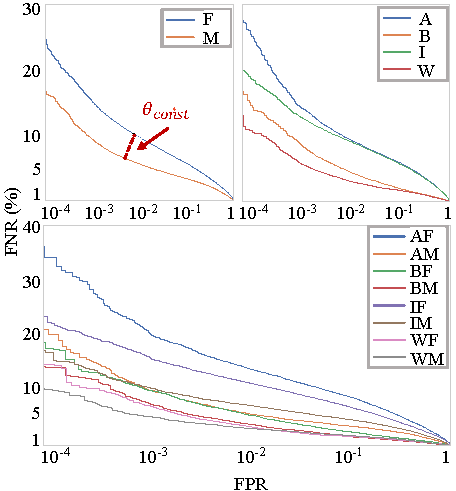
\includegraphics[width=.9\linewidth]{figures/detcurve-improved.pdf}
		\caption{\small{\textbf{\gls{det} curves.} \emph{Top-left}: per gender. \emph{Top-right}: per ethnicity. \emph{Bottom}: per subgroup (\ie combined). Dashed line shows about 2$\times$ difference in \gls{fpr} for the same threshold $\theta_{const}$. \gls{fnr} is the match error count (closer to the bottom is better).}}
		\glsreset{det}\glsreset{fpr}
\label{fig:detcurves} 
\end{figure} 
\vspace{1mm}
\noindent\textbf{Sampling faces and creating folds.} We created lists of pairs in five-folds with subjects split evenly per subject and without overlap across folds. Furthermore, a balance in the number of faces per was obtained by sampling twenty-five faces at random from each. Next, we generated a list of all the face pairs per subject, resulting in $\sum_{l=1}^{L}\sum_{k=1}^{K_d} {N_k \choose 2}$ positive pairs, where the number of faces of all $K_l$ subjects $N_k=25$  for each of the $L$ subgroups (Table~\ref{tab:ethnic-splits}). Next, we assigned subjects to a fold. To preserve balance across folds, we sorted subjects by the number of pairs and then started assigning to alternating folds from the one with the most samples. Note, this left no overlap in identity between folds. Later, a negative set from samples within the same subgroup randomly matched until the count met that of the positive. Finally, we doubled the number with negative pairs from across subgroups but in the same fold.


% \vspace{-5pt}
\subsection{Problem formulation}\label{subsec:pf} 
% \gls{lfw}~\cite{LFWTech}, a commonly used benchmark for ~\gls{fr}, reserves specific train-test face-pair lists. 
\Gls{fv} is the special case of the two-class (\ie boolean) classification. Hence, pairs are labeled as the ``same'' or ``different'' \textit{genuine} pairs (\ie \textit{match}) or \textit{imposter} (\ie \textit{mismatch}), respectively. This formulation (\ie \gls{fv}) is highly practical for applications like access control, re-identification, and surveillance. Typically, training a separate model for each unique subject is infeasible. Firstly, the computational costs compound as the number of subjects increase.  Secondly, such a scheme would require model retraining each time a new person is added. Instead, we train models to encode facial images in a feature space that captures the uniqueness of a face, to then determine the outcome based on the output of a scoring (or distance) function. Formally put:
\begin{equation}\label{eg:matcher}
    f_{boolean}(\vec{x}_i, \vec{x}_j) = d(\vec{x}_i, \vec{x}_j) \leq \theta,
\end{equation}

where $f_{boolean}$ is the \textit{matcher} of the feature vector $\vec{x}$ for the $i^{th}$ and $j^{th}$ sample~\cite{LFWTech}.

Cosine similarity is used as the \emph{matcher} in Eq~\ref{eg:matcher} the closeness of $i^{th}$ and $j^{th}$ features, \ie
$
s_l= \frac{f_i\cdot f_j}{||f_i||_2||f_j||_2}
$ is the closeness of the $l^{th}$ pair. 

\begin{figure}[t!] 
	\glsunset{fpr}
	\glsunset{sdm}
	\centering
	\centering
	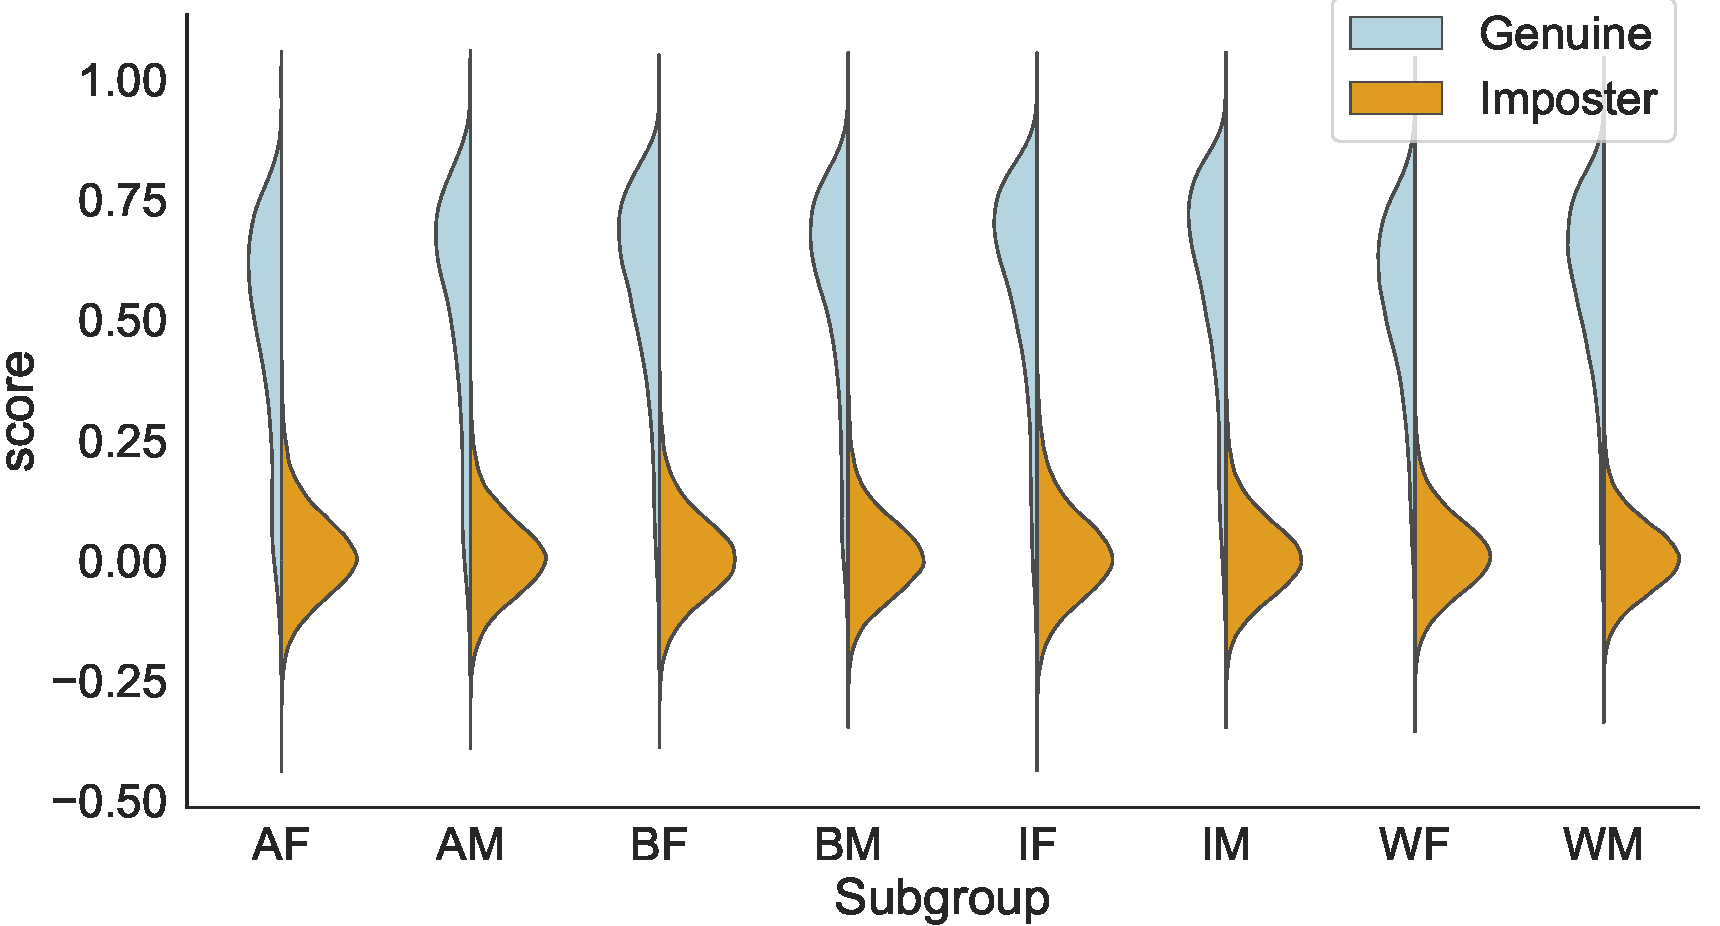
\includegraphics[width=1\linewidth]{figures/violinplots.pdf}
		\caption{\small{\textbf{\Gls{sdm} across subgroups.} Scores of \emph{imposters} have medians around 0.3 but with variations in upper percentiles; \emph{genuine} pairs vary in mean and spread (\eg \gls{af} has more area of overlap). A threshold varying across different subgroups yields a constant \gls{fpr}.}} \label{fig:detection-model} 
		\glsreset{sdm}
\end{figure} 

\subsection{Human assessment}\label{subsec:human-assessment}
We evaluated human on face pairs focusing on two racial groups: Chinese and Caucasians. To focus on the experiment, we honed-in on two groups, white Americans (W) and Chinese from China (C). The purpose was to minimize variability by only analyzing the subsets of the broader groups of whites and Asians. 

Samples were collected by recruiting subjects from multiple sources (\eg social media, email lists, and family/friends)-- a total of 120 participants were sampled at random from all the submissions that were (1) complete and (2) from a W or C participant. Specifically, there were 60 W and 60 C, both with \gls{m} and \gls{f} split evenly. A total of 50 face pairs of non-famous ``look-alikes'' were collected from the internet, with 20 ({\emph WA}) and 20 ({\emph C}) pairs (male and female split evenly). The other 10 pairs are of others (\eg Hispanic/ Latino, Japanese, African). The survey was created, distributed, and recorded via \href{https://paperform.co}{PaperForm}. 


\begin{figure}[t!]
	\centering    
	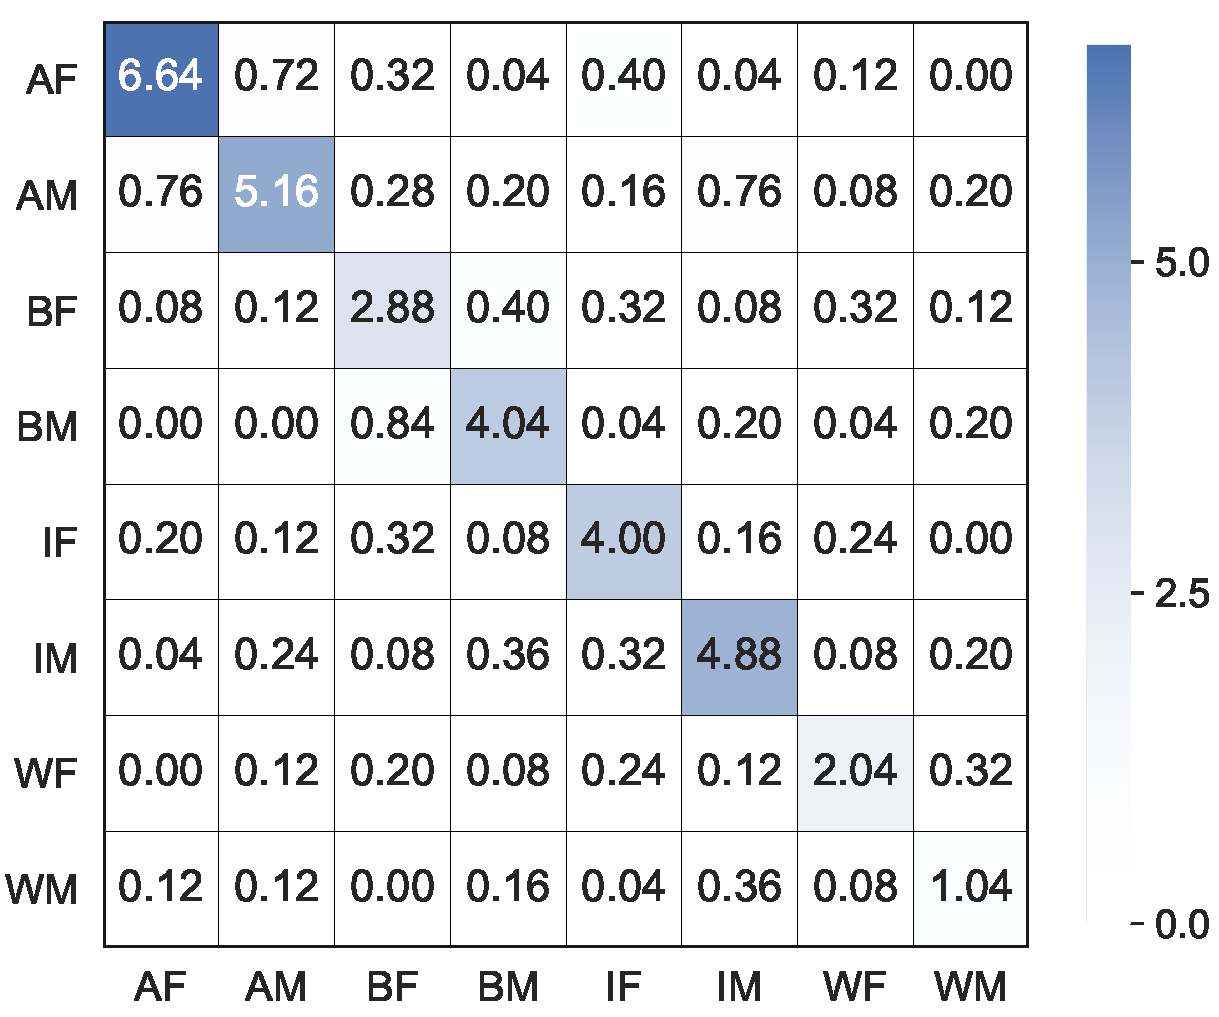
\includegraphics[width=.75\linewidth]{figures/confusion.pdf}
		\caption{\small{\textbf{Confusion matrix.} Percent error (Rank 1, \%) for all faces of \gls{bfw} versus all others. Error concentrates within a subgroup - consistent with the \gls{sdm} (Fig.~\ref{fig:detection-model}), as \gls{af} performs the worst, confusing mostly within subgroup. This plot is evidence that while race/ethnicity may be challenging to define, the subgroups are meaningful.}}
		\label{fig:confusion} 
\end{figure} 

\section{Results and Analysis}
A single \gls{cnn} was used as a means to control the experiments. For this, Sphereface~\cite{liu2017sphereface} trained on CASIA-Web~\cite{yi2014learning}, and evaluated on \gls{lfw}~\cite{LFWTech} (\%99.22 accuracy), encoded all of the faces.\footnote{\href{$https://github.com/clcarwin/sphereface\_pytorch$}{https://github.com/clcarwin/sphereface\_pytorch}} As reported in~\cite{wang2019racial}, \gls{lfw} has about a 13\%, 14\%, 3\%, and 70\% ratio in Asians, Blacks, Indians, and Whites, respectively; furthermore, CASIA-Web is even more unbalanced (again, as reported in~\cite{wang2019racial}), with about  3\%, 11\%, 2\%, and 85\% for the same subgroups.


% Specifically, we analyze three \glspl{cnn} variants: we encode faces using VGG-16~\cite{simonyan2014very},  50-layer residual network (\ie ResNet-50)~\cite{he2016deep}, and \gls{senet} (\ie SENet-50)~\cite{hu2018squeeze}, with results of only the latter (\ie the best performing \gls{senet}) model used throughout the main paper. Results for the other two, alongside \gls{senet} for comparison, are in the Supplemental Material.


\glsunset{am}\glsunset{af}\glsunset{bm}\glsunset{bf}\glsunset{im}\glsunset{if}\glsunset{wm}\glsunset{wf}

\subsection{Score analysis}
Fig.~\ref{fig:detection-model} shows score distributions for faces of the same (\ie \emph{Genuine}) and different (\ie \emph{Imposter}) identity, with a subgroup per \gls{sdm} plot. Notice that score distributions for imposters tend to peak about zero for all subgroups, and with minimal deviation comparing modes of the different plots. On the other hand, the score distribution of the \emph{genuine} pairs varies across subgroups in location (\ie score value) and spread (\ie overall shape). Asian Fem
Fig.~\ref{fig:confusion} shows the confusion matrix of the subgroups. A vast majority of errors occur in the intra-subgroup. It is interesting to note that while the definition of  each group  based on ethnicity and race may not be crisply defined, the confusion matrix indicates that in practice the \gls{cnn} finds that the groups are effectively separate. The categories are, therefore, meaningful in the context of \gls{fr}.

\begin{figure}[t!]
 
    % \begin{subfigure}[t]{\linewidth}
    
       \centering
%     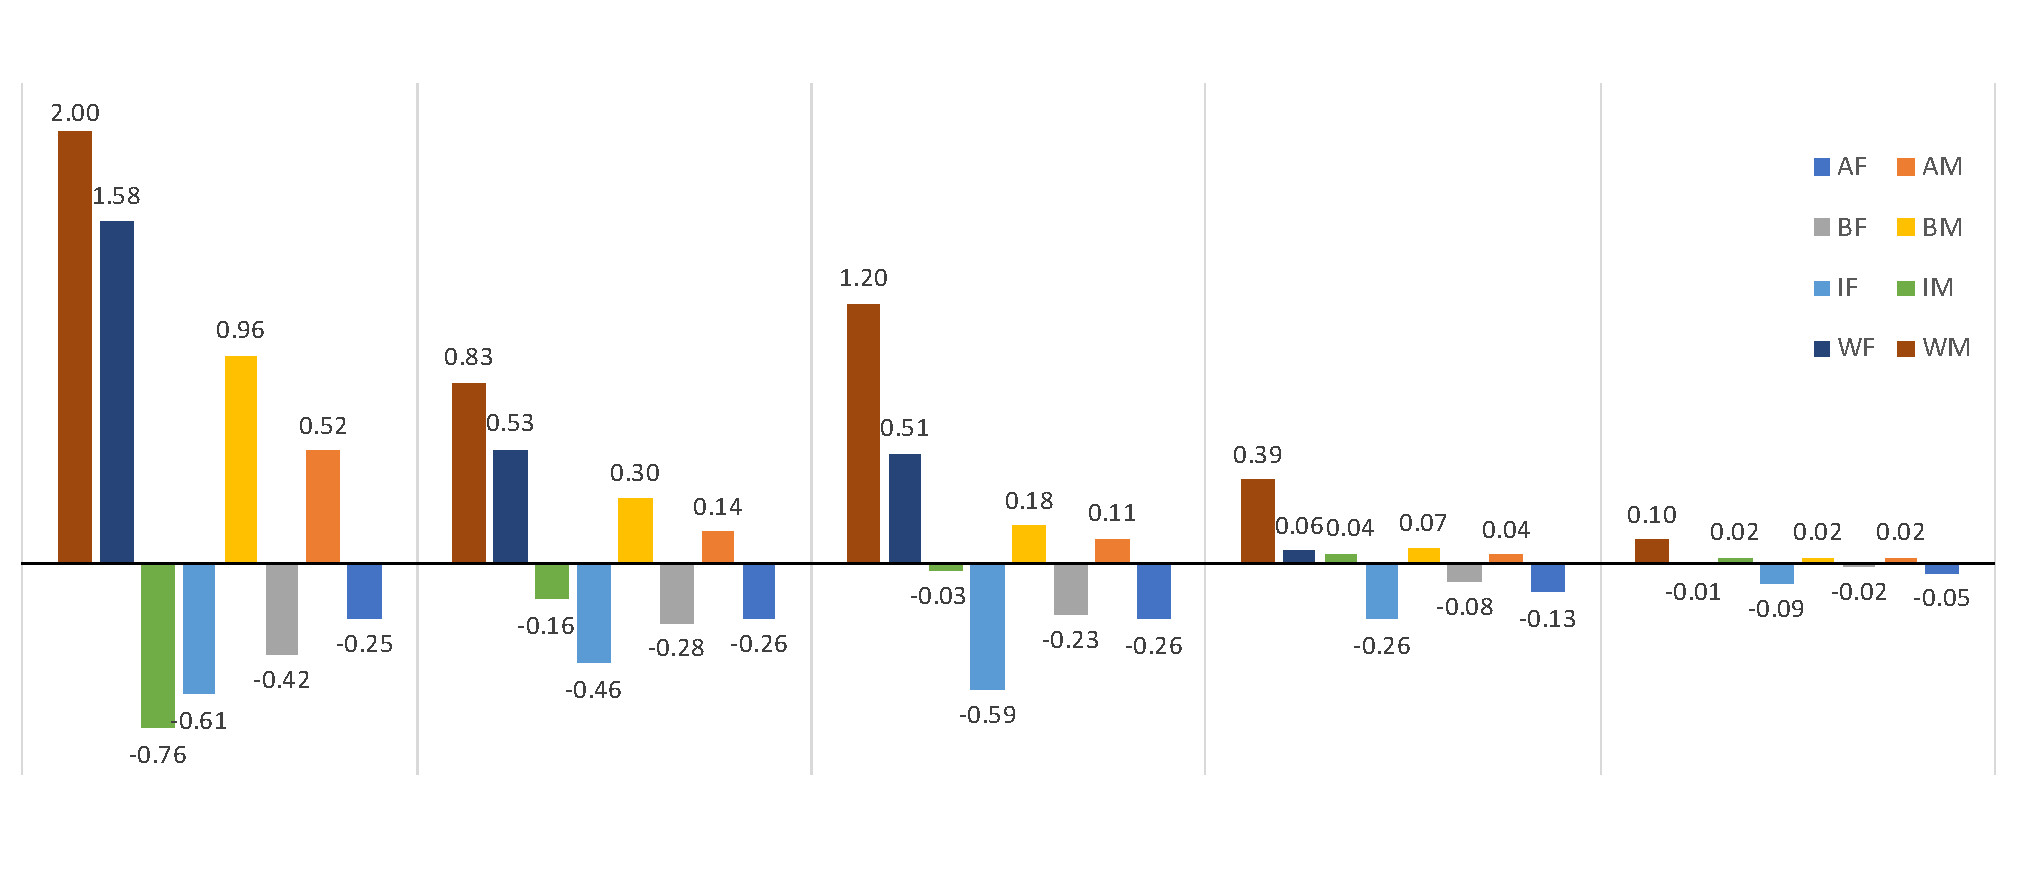
\includegraphics[width=.85\linewidth]{figures/global_threshold_fpr_percent_diff.pdf}
%     \caption{Global threshold ($t_g$)}
%  \end{subfigure}
%     \begin{subfigure}[t]{\linewidth}
%       \centering
    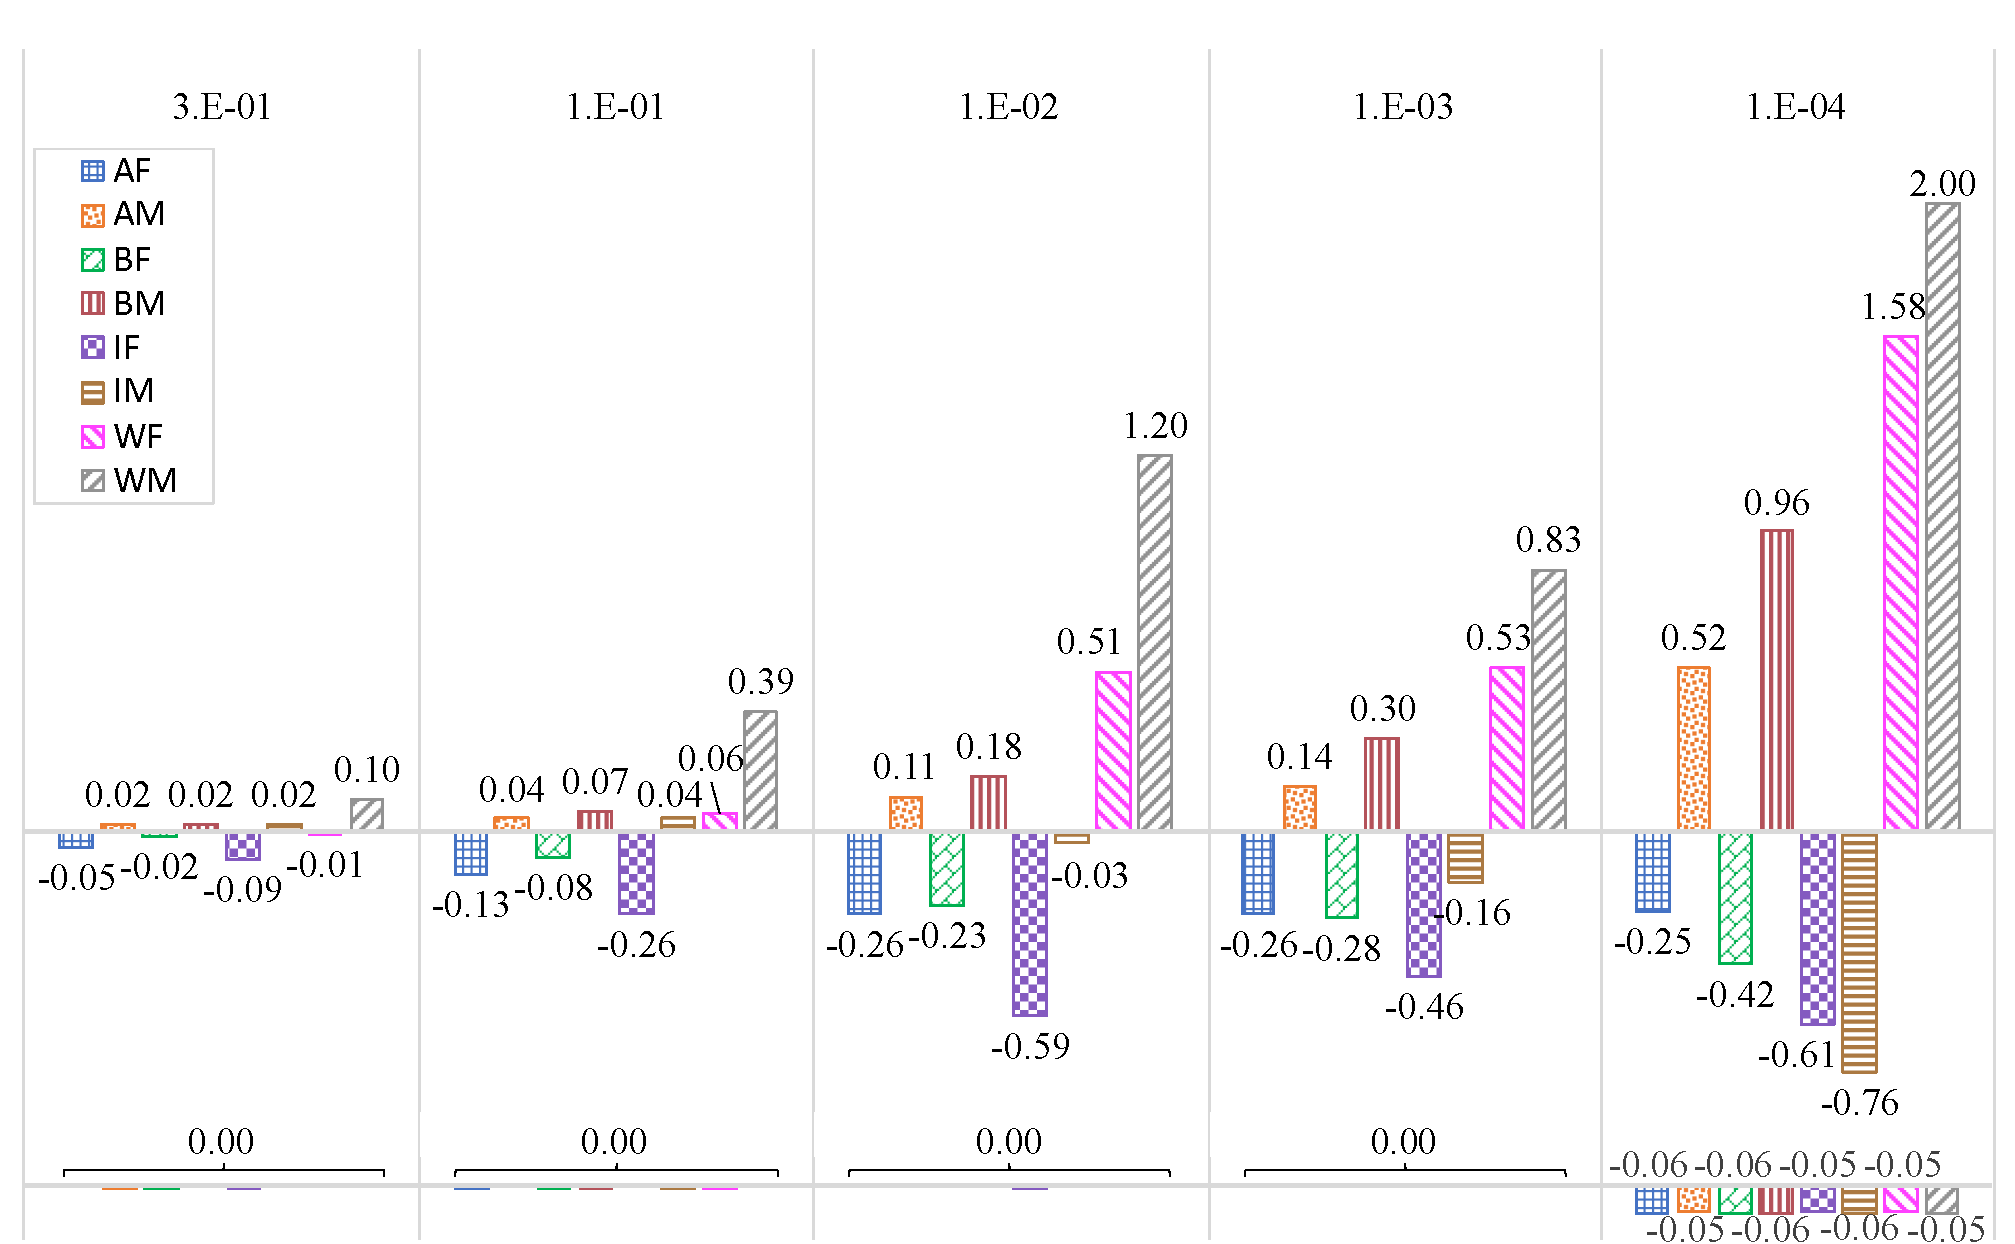
\includegraphics[width=.95\linewidth]{figures/adaptive_fpr_percent_diff_complete.pdf}
    % \caption{Optimal threshold ($t_o$)}
%   \end{subfigure}
    \caption{\small{\textbf{Percent difference from intended \gls{fpr}.} \emph{Top:} $t_g$ yields \gls{fpr} the span as large as 2$\times$ (\ie 200\%) that intended (\ie \gls{wm} for 1e-4). Furthermore, \gls{f} subgroups tend to perform worse than intended for all cases (while \gls{m} tend to overshoot intended performance, with exception of \gls{im} in for \gls{fpr}=1e-4). \emph{Bottom:} Subgroup-specific thresholds reduces this difference to near zero, where there are small differences, the percent difference across different subgroups is fair (\ie FPR=1e-4).}}\label{fig:percent:difference}
\end{figure}
\subsection{\gls{det} analysis}
\glsunset{m}
\glsunset{f}

\begin{figure*}[h!]
    \centering
    \begin{subfigure}[t]{.3\linewidth}
    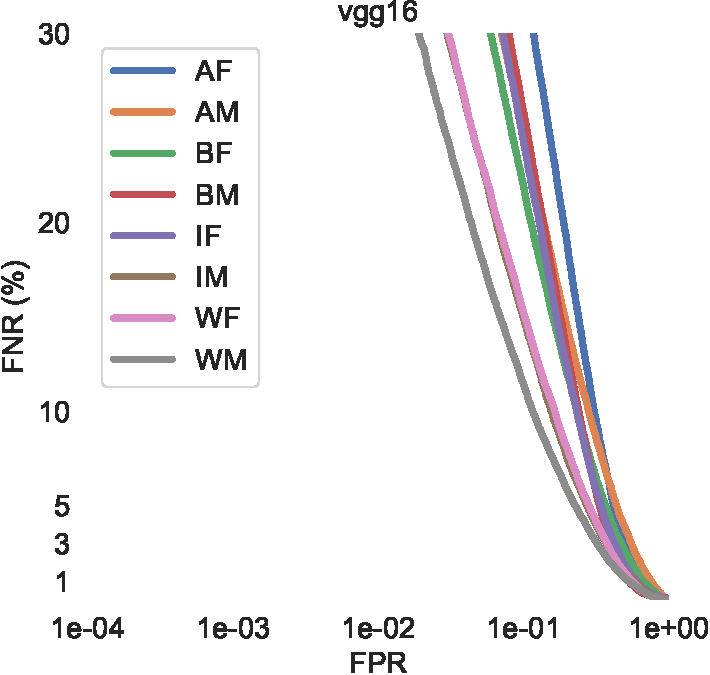
\includegraphics[width=.71\linewidth]{figures/curve_vgg16_subgroups-crop.pdf}
    \caption{VGG16~\cite{simonyan2014very}}
 \end{subfigure}
    \begin{subfigure}[t]{.27\linewidth}
    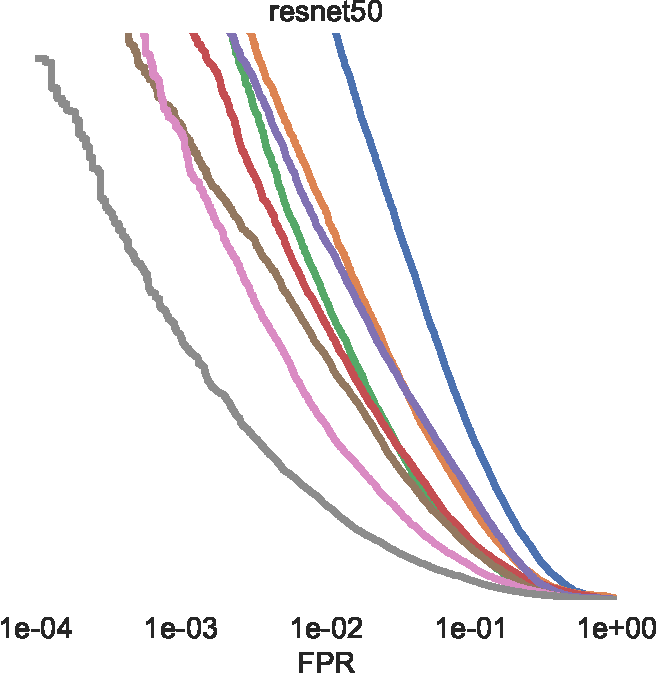
\includegraphics[width=.75\linewidth]{figures/curve_resnet50_subgroups-crop.pdf}
    \caption{ResNet50~\cite{he2016deep}}
   \end{subfigure}
    \begin{subfigure}[t]{.27\linewidth}
    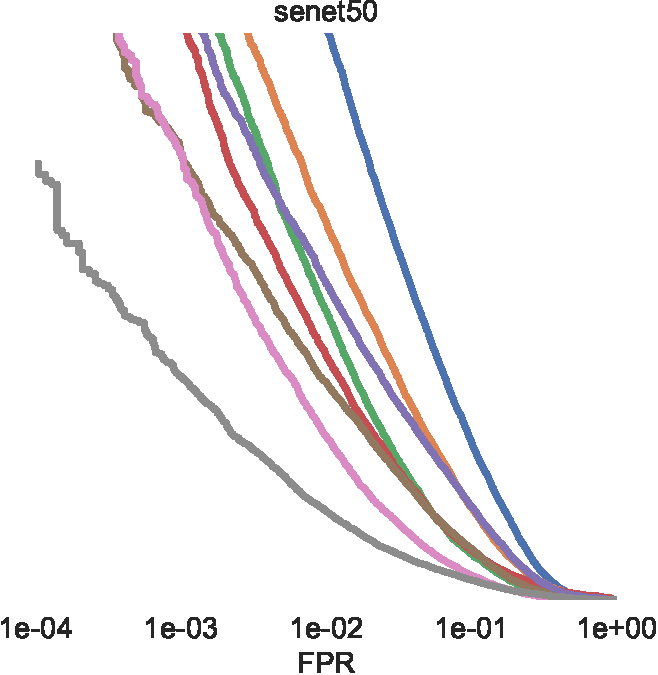
\includegraphics[width=.75\linewidth]{figures/curve_senet50_subgroups-crop.pdf}
    \caption{SENet~\cite{hu2018squeeze}}
    \end{subfigure}
    \caption{\small{\textbf{\gls{det} curves for different CNNs}. \gls{fnr} (\%) (vertical) vs \gls{fpr}  (horizontal, log-scale) for VGG2~\cite{Cao18} models with different backbones (VGG16, Resnet50, SEnet50). Lower is better. For each plot, \gls{wm} is the top-performer, while \gls{af} is the worst. The the ordering of the curves is roughly the same for each backbone.}}\label{fig:sdm-appendix-a}
\end{figure*}




\gls{det} curves averaged across 5-folds show per-subgroup trade-offs (Fig.~\ref{fig:detcurves}). Note that \gls{m} performs better than \gls{f}, precisely as one would expect from the tails of score-distributions for \emph{genuine} pairs (Fig.~\ref{fig:detection-model}). \Gls{af} and \gls{if} perform the worst.


 
\begin{table}[b!]
\glsunset{tar}
\glsunset{far}
\caption{\small{\textbf{\gls{tar} at intervals of \gls{far}}. gls{far}, listed are the \gls{tar} scores for a global threshold (top) and the proposed category-based threshold (bottom). Higher is better.}}\label{tab:ethnicy-far} 
%  \vspace{-2mm}
\begin{center}
\scriptsize
\begin{tabular}{l c c c c c}
     \gls{far} & 0.3 & 0.1 & 0.01 & 0.001 & 0.0001\\\midrule
    \multirow{2}{.1mm}{\textbf{\gls{af}}} &0.990 & 0.867 & 0.516 & 0.470 & 0.465\\[-4pt]
        &1.000 & 0.882 & 0.524 & 0.478 & 0.474\\[-1pt]
    \multirow{2}{3mm}{\textbf{\gls{am}}} &0.994 & 0.883 & 0.529 & 0.482 & 0.477\\[-4pt]
        &1.000 & 0.890 & 0.533 & 0.486 & 0.482\\[-1pt]
    \multirow{2}{3mm}{\textbf{\gls{bf}}} &0.991 & 0.870 & 0.524 & 0.479 & 0.473\\[-4pt]
        &1.000 & 0.879 & 0.530 & 0.484 & 0.480\\[-1pt]
    \multirow{2}{3mm}{\textbf{\gls{bm}}} &0.992 & 0.881 & 0.526 & 0.480 & 0.474\\[-4pt]
        &1.000 & 0.891 & 0.532 & 0.485 & 0.480\\[-1pt]
    \multirow{2}{3mm}{\textbf{\gls{if}}} &0.996 & 0.881 & 0.532 & 0.486 & 0.481\\[-4pt]
        &1.000 & 0.884 & 0.534 & 0.488 & 0.484\\[-1pt]
    \multirow{2}{3mm}{\textbf{\gls{im}}} &0.997 & 0.895 & 0.533 & 0.485 & 0.479\\[-4pt]
        &1.000 & 0.898 & 0.535 & 0.486 & 0.481\\[-1pt]
    \multirow{2}{3mm}{\textbf{\gls{wf}}} &0.988 & 0.878 & 0.517 & 0.469 & 0.464\\[-4pt]
        &1.000 & 0.894 & 0.526 & 0.478 & 0.474\\[-1pt]
    \multirow{2}{3mm}{\textbf{\gls{wm}}} &0.989 & 0.896 & 0.527 & 0.476 & 0.470\\[-4pt]
        &1.000 & 0.910 & 0.535 & 0.483 & 0.478\\[-1pt]
    \midrule
    \multirow{2}{3mm}{\textbf{Avg.}} &0.992 & 0.881 & 0.526 & 0.478 & 0.474\\[-4pt]
        &1.000 & 0.891 & 0.531 & 0.483 & 0.479\\[-10pt]
\end{tabular}
\end{center}
\glsreset{tar}
\glsreset{far}
%  \vspace{-3mm}

\end{table}


The gender-based \gls{det} curve shows a difference in performances between \gls{m} and \gls{f} with a fixed threshold (dashed line). Similar effects exist for the other curves as well (lines omitted to declutter). For many \gls{fr} applications, systems are operated at the highest \gls{fpr} allowed, so the line of constant threshold indicates that a single threshold produces different operating points (\ie \gls{fpr}), which is undesirable.  The difference in \gls{fpr} is approximately a factor of two-- quite large indeed. If this is the case in an industrial system, one would expect a difference in about double the false positives to be reported based on subgroup alone. The potential ramifications of such a bias should not be overlooked, which it has not as of lately-- gaining the interest in even main-stream media ~\cite{england2019,snow2018}.

% \subsubsection{Other \gls{cnn} models.}~\label{app:sec:other:models}
Variations in optimal threshold exist across models (Fig.~\ref{fig:sdm-appendix-a}). Like in Fig.~\ref{fig:detcurves}, the \gls{det} curves for three \gls{cnn}-based models, each trained on VGG2 with softmax but with different backbones.\footnote{\href{https://github.com/rcmalli/keras-vggface}{https://github.com/rcmalli/keras-vggface}} Notice similar trends across subgroups and models, which is consistent with  Sphereface as well (Fig.~\ref{fig:detcurves}). For example, the plots generated with Spherface and VggFace2 all have the \gls{wm} curve at the bottom (\ie best) and \gls{af} on top (\ie worst). Thus, the additional \gls{cnn}-based models demonstrate the same phenomena: proportional to the overall model performance, exact in which the ordering subgroups insensitivity in scores space.

\subsection{Verification threshold} \label{subsec:analysis:verification}
We seek to reduce the bias between subgroups. Such that an operating point (\ie \gls{fpr}) is constant across subgroups. To accomplish that, we used a per subgroup threshold. In \gls{fv}, we consider one image as the query and all others as the test. For this, the ethnicity of the query image is assumed. We can then examine the \gls{det} curves and pick the best threshold per subgroup for a certain \gls{fpr}.

We evaluated \gls{tar} for specific \gls{far} values. As described in Section~\ref{subsec:pf}, the verification experiments were 5-fold, with no overlap in subject ID between folds. Results reported are averaged across folds in all cases and are shown in Table~\ref{tab:ethnicy-far}. For each subgroup, the \gls{tar} of using a global threshold is reported (upper row), as well as using the optimal per subgroup threshold (lower row). 

Even for lower \gls{far}, there are notable improvements, often of the order of 1\%, which can be challenging to achieve when \gls{far} is near $\geq$90\%. More importantly, each subgroup has the desired \gls{fpr}, so that substantial differences in \gls{fpr} will remain unfounded. We experimented with ethnicity estimators on both the query and test image, which yielded similar results to those reported here.

%%%%%%%%%%%%%%%%%%%%%%%%%%%%%%%%%%%%%%%%%%%%%%%%%%%%%%%%%%%%%%%%%%%%%%%%%%%%%%%%
\begin{table}[t!]
\begin{center}
    \caption{\small{\textbf{Human assessment (quantitative).} Subgroups listed per row (\ie human) and column (\ie image). Note, most do the best intra-subgroup (\textcolor{blue}{blue}), and second-best (\textcolor{red}{red}) intra-subgroup but inter-gender. WF performs the best; WF pairs are most correctly matched.}}
    % CF shows the least variation, but with the lowest accuracy. WF shows the best accuracy, in human performance and on face pairs of that subgroup.}}
    \label{tab:humsn-eval-results} 
    % \vspace{-5mm}
    %  \vspace{-2mm}
\footnotesize
\scalebox{0.94}{
\begin{tabular}{c}
\begin{tabular}{c l c c c cc}
&&\multicolumn{4}{c}{\textbf{Image}}\\
   \multicolumn{2}{c}{(Acc, \%)}& CF  & CM & WF &WM& Avg\\
\end{tabular}\\
\begin{tabular}{c l| r r r r| r}
\cline{3-7}
       &CF &\  \textbf{\textcolor{blue}{52.9}}&   \textbf{\textcolor{red}{48.0}}&43.8&44.7 &47.4 \\
         \multirow{\items}{*}{\rotatebox{90}{\textbf{Human}}} \hspace{-5mm}
        &CM &  \textbf{\textcolor{red}{45.6}} & \textbf{\textcolor{blue}{50.4}}  & 44.4 &36.2 &44.1 \\
       
        &WF & 44.7 &43.8 & \textbf{\textcolor{blue}{57.3}}& \textbf{\textcolor{red}{48.0}} & \textbf{48.5} \\
        &WM & 30.1&\textbf{\textcolor{red}{47.4}} &  45.3 & \textbf{\textcolor{blue}{56.1}} & 44.7\\\cline{3-7}
        &Avg &  43.3& 47.4&\textbf{47.7} &46.3 &46.2\\
 \end{tabular}
 \end{tabular}
 }
 
 \end{center}
%  \vspace{-7mm}
\end{table} 


\subsection{Human evaluation}
Subjects of a subgroup likely have mostly been exposed to others of the same (Table~\ref{tab:humsn-eval-results} and Fig.~\ref{fig:human-eval}). Therefore, it is expected they would be best at labeling their own; similar for the same ethnicity, but another gender. Our findings concur. Each subgroup is best at labeling their type, and then second best at labeling the same ethnicity but opposite sex. Interestingly, each group of images is best tagged by the corresponding subgroup, with the second-best having the same ethnicity and opposite gender. On average, subgroups are comparable at labeling images. Analogous to the \gls{fr} system, performance ratings differ when analyzing within and across subgroups. In other words, performance on \gls{bfw} improved with subgroup-specific thresholds. Similarly, humans tend to better recognize individuals by facial cues of the same or similar demographics. Put differently, as the recognition performances drop with a global threshold optimized for one subgroup and deployed on another, human performance tends to drop when across subgroups (\ie most familiar intra-subgroup; a performance drop for other, less familiar subgroups).
 
%  for it better adapts wh specific to subgroup) shift in sensitivity across subgroups when deep encodings are compared, the underlying mechanism 

\begin{figure}[t!] 
	\centering    
	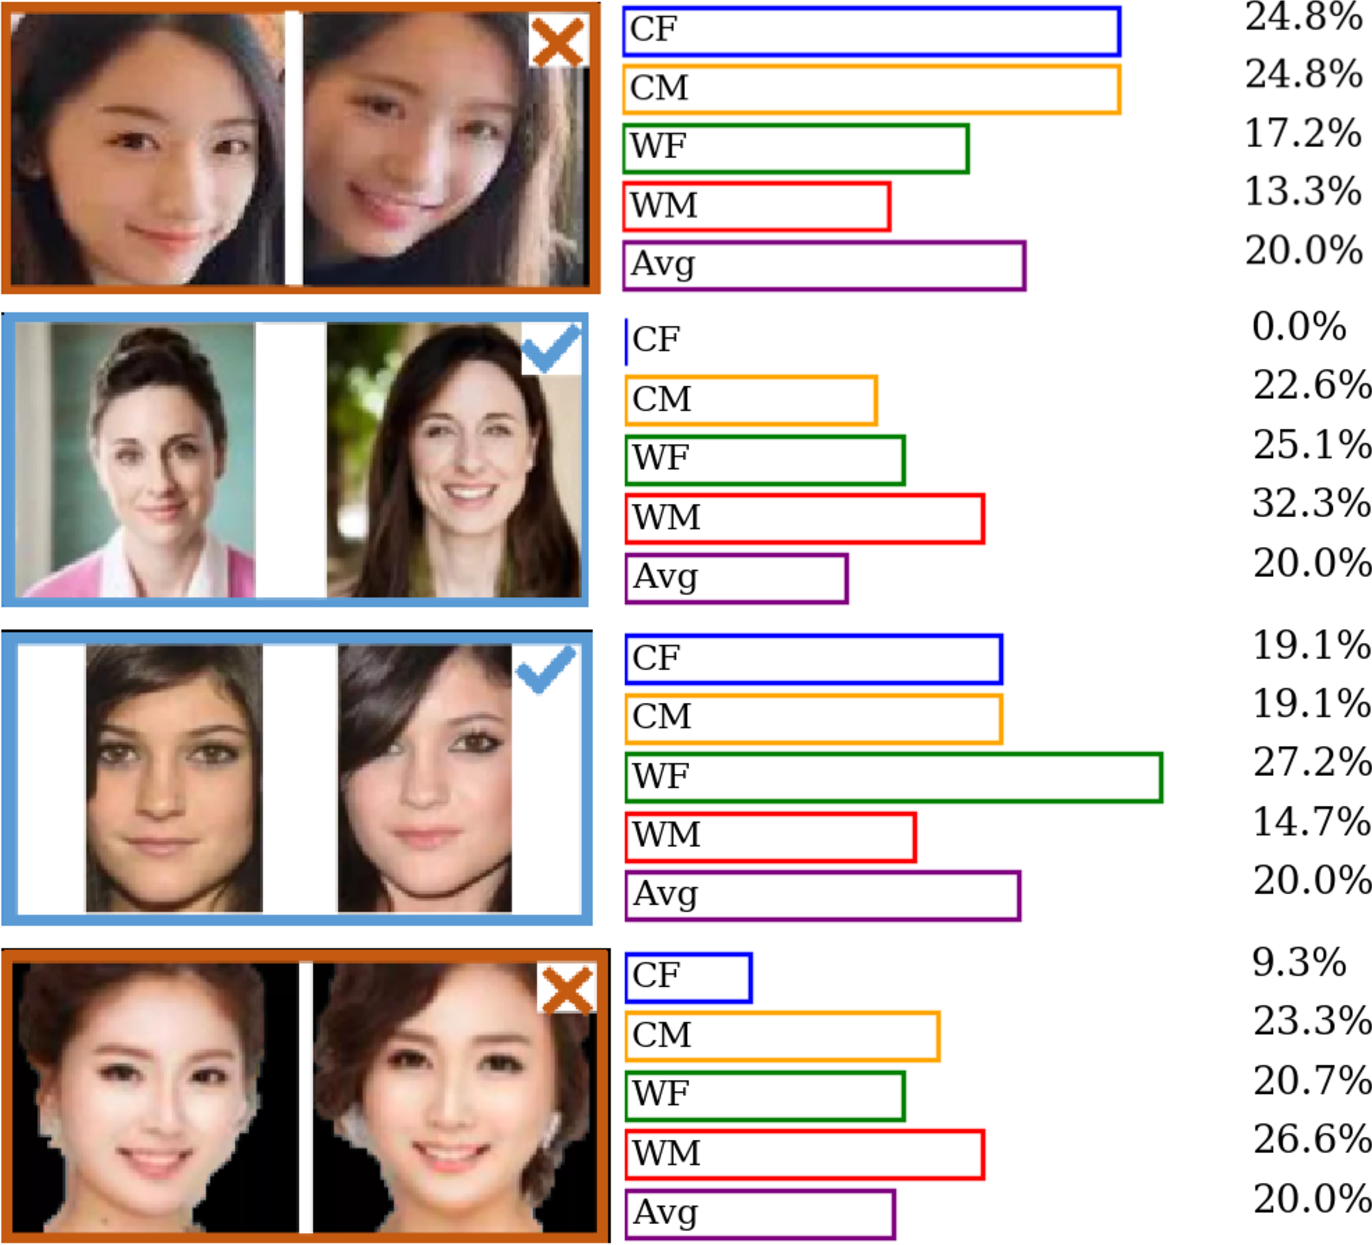
\includegraphics[width=.69\linewidth] {figures/human_eval.pdf}
		\caption{\small{\textbf{Human assessment (qualitative).} $\checkmark$ for \emph{match}; $\times$ for \emph{non-match}. Accuracy scores shown as bar plots. Humans are most successful at recognizing their own subgroup, with a few exceptions (\eg bottom).}}
		% (\eg bottom row). } Result summary in Table~\ref{tab:human-eval}.
		\label{fig:human-eval} 
% 		\vspace{-1mm}
\end{figure} 
% \vspace{-4mm}
% \vspace{-5pt}


% \scalebox{0.8}{
% \begin{tabular}{l c c c c c}
% \multicolumn{6}{c}{\textbf{Image}}\\
%         &  CF  &      CM     &   WF     &   WM     &  Avg\\\midrule
%         CF &  \textbf{\textcolor{blue}{52.9}}&   \textbf{\textcolor{red}{48.0}}&43.8&44.7 &47.4$\pm$4.1 \\
%         CM &  \textbf{\textcolor{red}{45.6}} & \textbf{\textcolor{blue}{0.504}}  & 44.4 &36.2 &44.1$\pm$5.9 \\
%         WF & 44.7 &43.8 & \textbf{\textcolor{blue}{0.573}}& \textbf{\textcolor{red}{48.0}} & 48.5$\pm$6.2 \\
%         WM & 30.1&\textbf{\textcolor{red}{47.4}} &  45.3 & \textbf{\textcolor{blue}{56.1}} & 44.7$\pm$10.8 \\\midrule
%         Avg &  43.3& 47.4&47.7 &46.3 &46.2$\pm$2.0\\
%  \end{tabular}}
%  \end{center}
% %  \vspace{-7mm}
% \end{table} 
% \newcommand\items{4}   %Number of classes
% \arrayrulecolor{white} %Table line colors
% \noindent\begin{tabular}{cc*{\items}{|E}|}
% \multicolumn{1}{c}{} &\multicolumn{1}{c}{} &\multicolumn{\items}{c}{Image} \\ \hhline{~*\items{|-}|}
% \multicolumn{1}{c}{} & 
% \multicolumn{1}{c}{} & 
% \multicolumn{1}{c}{CF} & 
% \multicolumn{1}{c}{{CM}} & 
% \multicolumn{1}{c}{{WF}}&
% \multicolumn{1}{c}{{WM}}\\ \hhline{~*\items{|-}|}
% \multirow{\items}{*}{\rotatebox{90}{Labeler}} 
% &Class A  & 100   & 0  & 10   \\ \hhline{~*\items{|-}|}
% &Class B  & 10   & 80  & 10   \\ \hhline{~*\items{|-}|}
% &Class C  & 30   & 0   & 70   \\ \hhline{~*\items{|-}|}
% &Class C  & 30   & 0   & 70   \\ \hhline{~*\items{|-}|}
% \end{tabular}

\glsresetall
\section{Conclusion}
We introduce a new data set \gls{bfw} with eight subgroups balanced across gender and ethnicity. With this, and upon highlighting the challenges and shortcomings of grouping subjects as a single subset, we provide evidence that forming subgroups is meaningful, as the FR algorithm rarely makes mistakes across subgroups. We used an \textit{off-the-shelf} Sphereface, hypothesizing this SOTA CNN suffers from bias because of the imbalanced train-set. Once established that the results do suffer from problems of bias, we observed that the same threshold across ethnic and gender subgroups leads to differences in the \gls{fpr} up to a factor of two. Furthermore, the percent difference from in which is seemingly the cause of the frenzy about bias in FR in main-stream media. Furthermore, we ameliorate these differences with a per-subgroup threshold, leveling out FPR, and achieving a higher TPR. We hypothesized that most humans grew amongst more than their own demographic and, therefore, effectively learn from imbalanced datasets-- a human evaluation validated that humans are biased, as most recognized their personal demographic best. The focused research findings presented here, along with the public database included, are extendable in vast ways. Thus, we see this as the slither to a much larger problem of bias in ML.



{\small
\bibliographystyle{ieee_fullname}
\bibliography{references}
}

% \putbib
% \end{bibunit}
% \begin{bibunit}
%
\newpage
\onecolumn
% \begin{minipage*}[\linewidth]{width of the minipage}
\renewcommand{\thesection}{\alph{section}}
\glsresetall
\setcounter{section}{0}

\section{Other \gls{cnn} models.}~\label{app:sec:other:models}
Variations in optimal threshold exist across models (Fig.~\ref{fig:sdm-appendix-a}). Like in Fig.~\ref{fig:detcurves}, the \gls{det} curves for three \gls{cnn}-based models, each trained on VGG2 with softmax but with different backbones.\footnote{Used pre-trained models and public Github, \href{https://github.com/rcmalli/keras-vggface}{https://github.com/rcmalli/keras-vggface}} Notice similar trends across subgroups and models, which is consistent with  Sphereface as well (Fig.~\ref{fig:detcurves}). For example, the plots generated with Spherface and VggFace2 all have the \gls{wm} curve at the bottom (\ie best) and \gls{af} on top (\ie worst). 
% ArcFace (not shown) shown similar results. We would have to cite + will incorporate later .... a blank statement and sphereface is comparable ... up to you i do not care
% \begin{figure}[h!]
% % \vspace{-2mm}
%     \centering
%     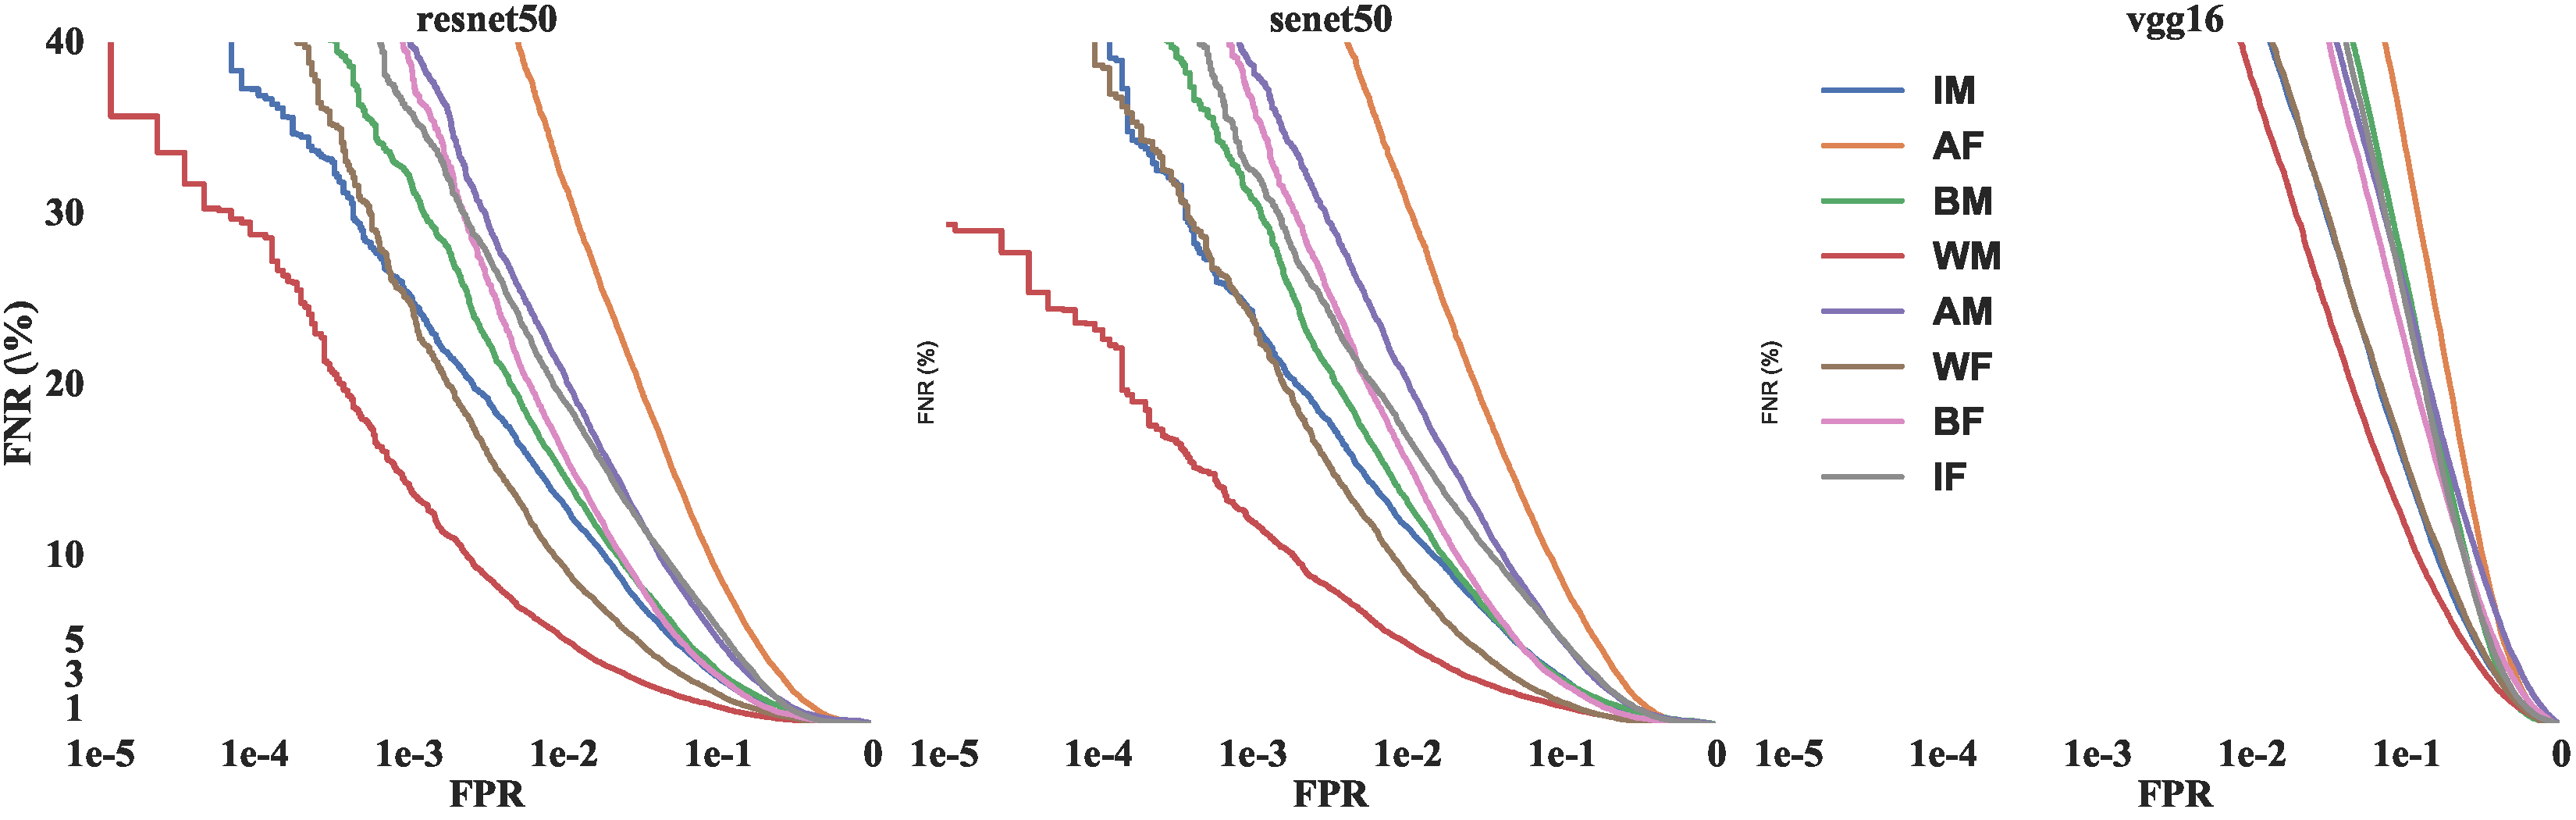
\includegraphics[width=.8\linewidth, trim={0mm 0mm 0mm 0mm},clip]{figures/SDM.pdf}\\
%     \caption{\textbf{\gls{det} curves for different CNN models}. \gls{fnr} (\%) (vertical) vs \gls{fpr} (log-scale)  (horizontal) for VGG2~\cite{Cao18} models with different backbones (vgg16, Resnet50~\cite{he2016deep}, SEnet50~\cite{hu2018squeeze}). Lower is better. For each plot, \gls{wm} is the best performing curve, \gls{af} is the worst. The the ordering of the curves is roughly the same for each backbone.}\label{fig:sdm-appendix-a}
%     \vspace{-3mm}
% \end{figure}


\begin{figure}[h!]
\vspace{-1mm}
    \centering
    \begin{subfigure}[t]{.3\linewidth}
    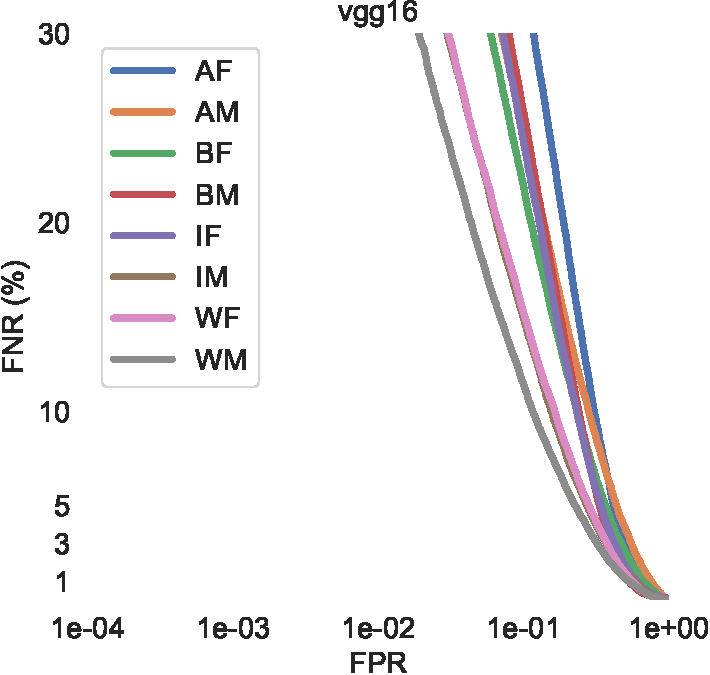
\includegraphics[width=.75\linewidth]{figures/curve_vgg16_subgroups-crop.pdf}
    \caption{VGG16~\cite{simonyan2014very}}
 \end{subfigure}
    \begin{subfigure}[t]{.27\linewidth}
    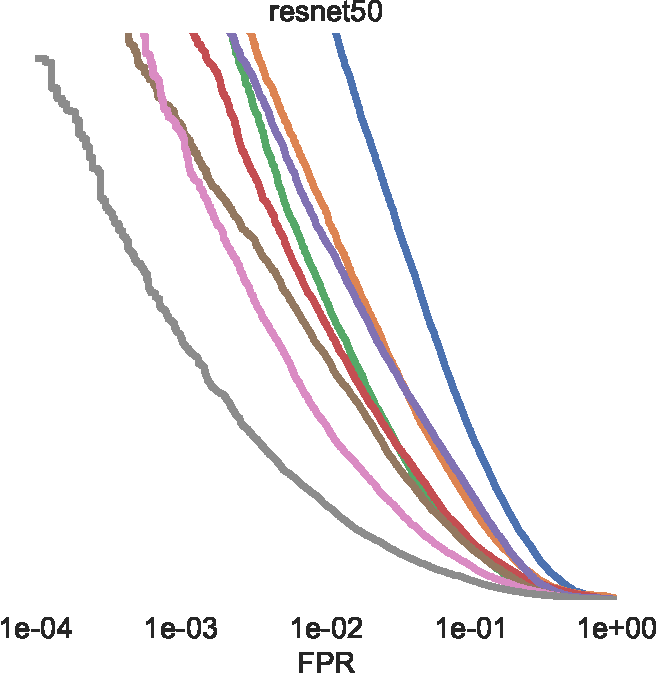
\includegraphics[width=.8\linewidth]{figures/curve_resnet50_subgroups-crop.pdf}
    \caption{ResNet50~\cite{he2016deep}}
   \end{subfigure}
    \begin{subfigure}[t]{.27\linewidth}
    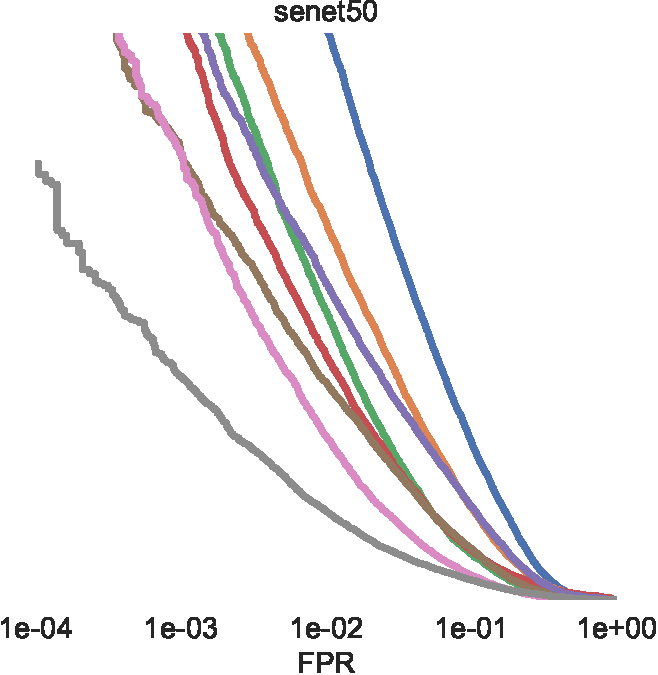
\includegraphics[width=.8\linewidth]{figures/curve_senet50_subgroups-crop.pdf}
    \caption{SENet~\cite{hu2018squeeze}}
    \end{subfigure}
    \caption{\textbf{\gls{det} curves for different CNN models}. \gls{fnr} (\%) (vertical) vs \gls{fpr} (log-scale)  (horizontal) for VGG2~\cite{Cao18} models with different backbones (VGG16, Resnet50, SEnet50). Lower is better. For each plot, \gls{wm} is the best performing curve, \gls{af} is the worst. The the ordering of the curves is roughly the same for each backbone.}\label{fig:sdm-appendix-a}
    \vspace{-1mm}
\end{figure}



Sample faces per subgroup of the \gls{bfw} dataset are shown in Fig.~\ref{fig:montage:app}.
\begin{figure}[h!]
\vspace{-2mm}
    \centering
    \includegraphics[width=.7\linewidth]{figures/facemontage.pdf}
    \caption{\textbf{Sample of \gls{bfw}}. Each row depicts a different gender, \gls{f} (top) and \gls{m} (bottom). Columns are grouped by ethnicity (\ie \gls{a}, \gls{b}, \gls{i}, and \gls{w}, respectfully).}
    \label{fig:montage:app}
    \vspace{-1mm}
\end{figure}
{
\scriptsize
\begin{thebibliography}{widest entry}
 \bibitem[1]{Cao18} Qiong Cao, Li Shen, Weidi Xie, Omkar M. Parkhi, and Andrew Zisserman. ``Vggface2: A dataset for recognising faces across pose and age.'' In \textit{IEEE International Conference on Automatic Face \& Gesture Recognition.} 2018.
 \bibitem[2]{simonyan2014very} Karen Simonyan and Andrew Zisserman. ``Very deep convolutional networks for large-scale image recognition'' \textit{arXiv preprint arXiv:1409.1556.} 2014.
  \bibitem[3]{he2016deep} He, Kaiming, Xiangyu Zhang, Shaoqing Ren, and Jian Sun. ``Deep residual learning for image recognition.'' In \textit{IEEE Conference on Computer Vision and Pattern Recognition.} 2016.
 \bibitem[4]{hu2018squeeze} Hu, Jie, Li Shen, and Gang Sun. ``Squeeze-and-excitation networks.'' In \textit{IEEE Conference on Computer Vision and Pattern Recognition.} 2018.
\end{thebibliography}
}

% \end{minipage*}
% \end{bibunit}

\end{document}
